\section*{\begin{tabular*}{\linewidth}{@{}l @{\extracolsep{\fill}} r@{}}
Nr.~8 & PIK~87/1 \\
\end{tabular*} 
}

\textsf{\textbf{Pikunda (\mbox{Sangha}; Fpl.~255)}}

\vspace{1em}

\noindent\begin{tabular}{@{}rl@{}}
\textbf{Feldarbeit:} & \begin{tabular}[t]{@{}l@{}}\textbf{03.06.--13.06.1987}\\ \textbf{(M. K. H. Eggert)}\end{tabular} \\ 
\textbf{Abb.:} & \textbf{\ref{fig:PIK87_Fundstelle}--\ref{fig:PIK87_Datierungen}} \\ 
\textbf{Tab.:} & \textbf{\ref{tab:PIK87-1_Befunde}--\ref{tab:PIK87-1_Datierungen}}\\
\textbf{Taf.:} & \textbf{44.3--48.16} \\ 
\textbf{Lit.:} & \textbf{\textsc{Eggert}~1992, 1993} \\ 
\end{tabular} 

\begin{figure*}[tb]
 \centering
 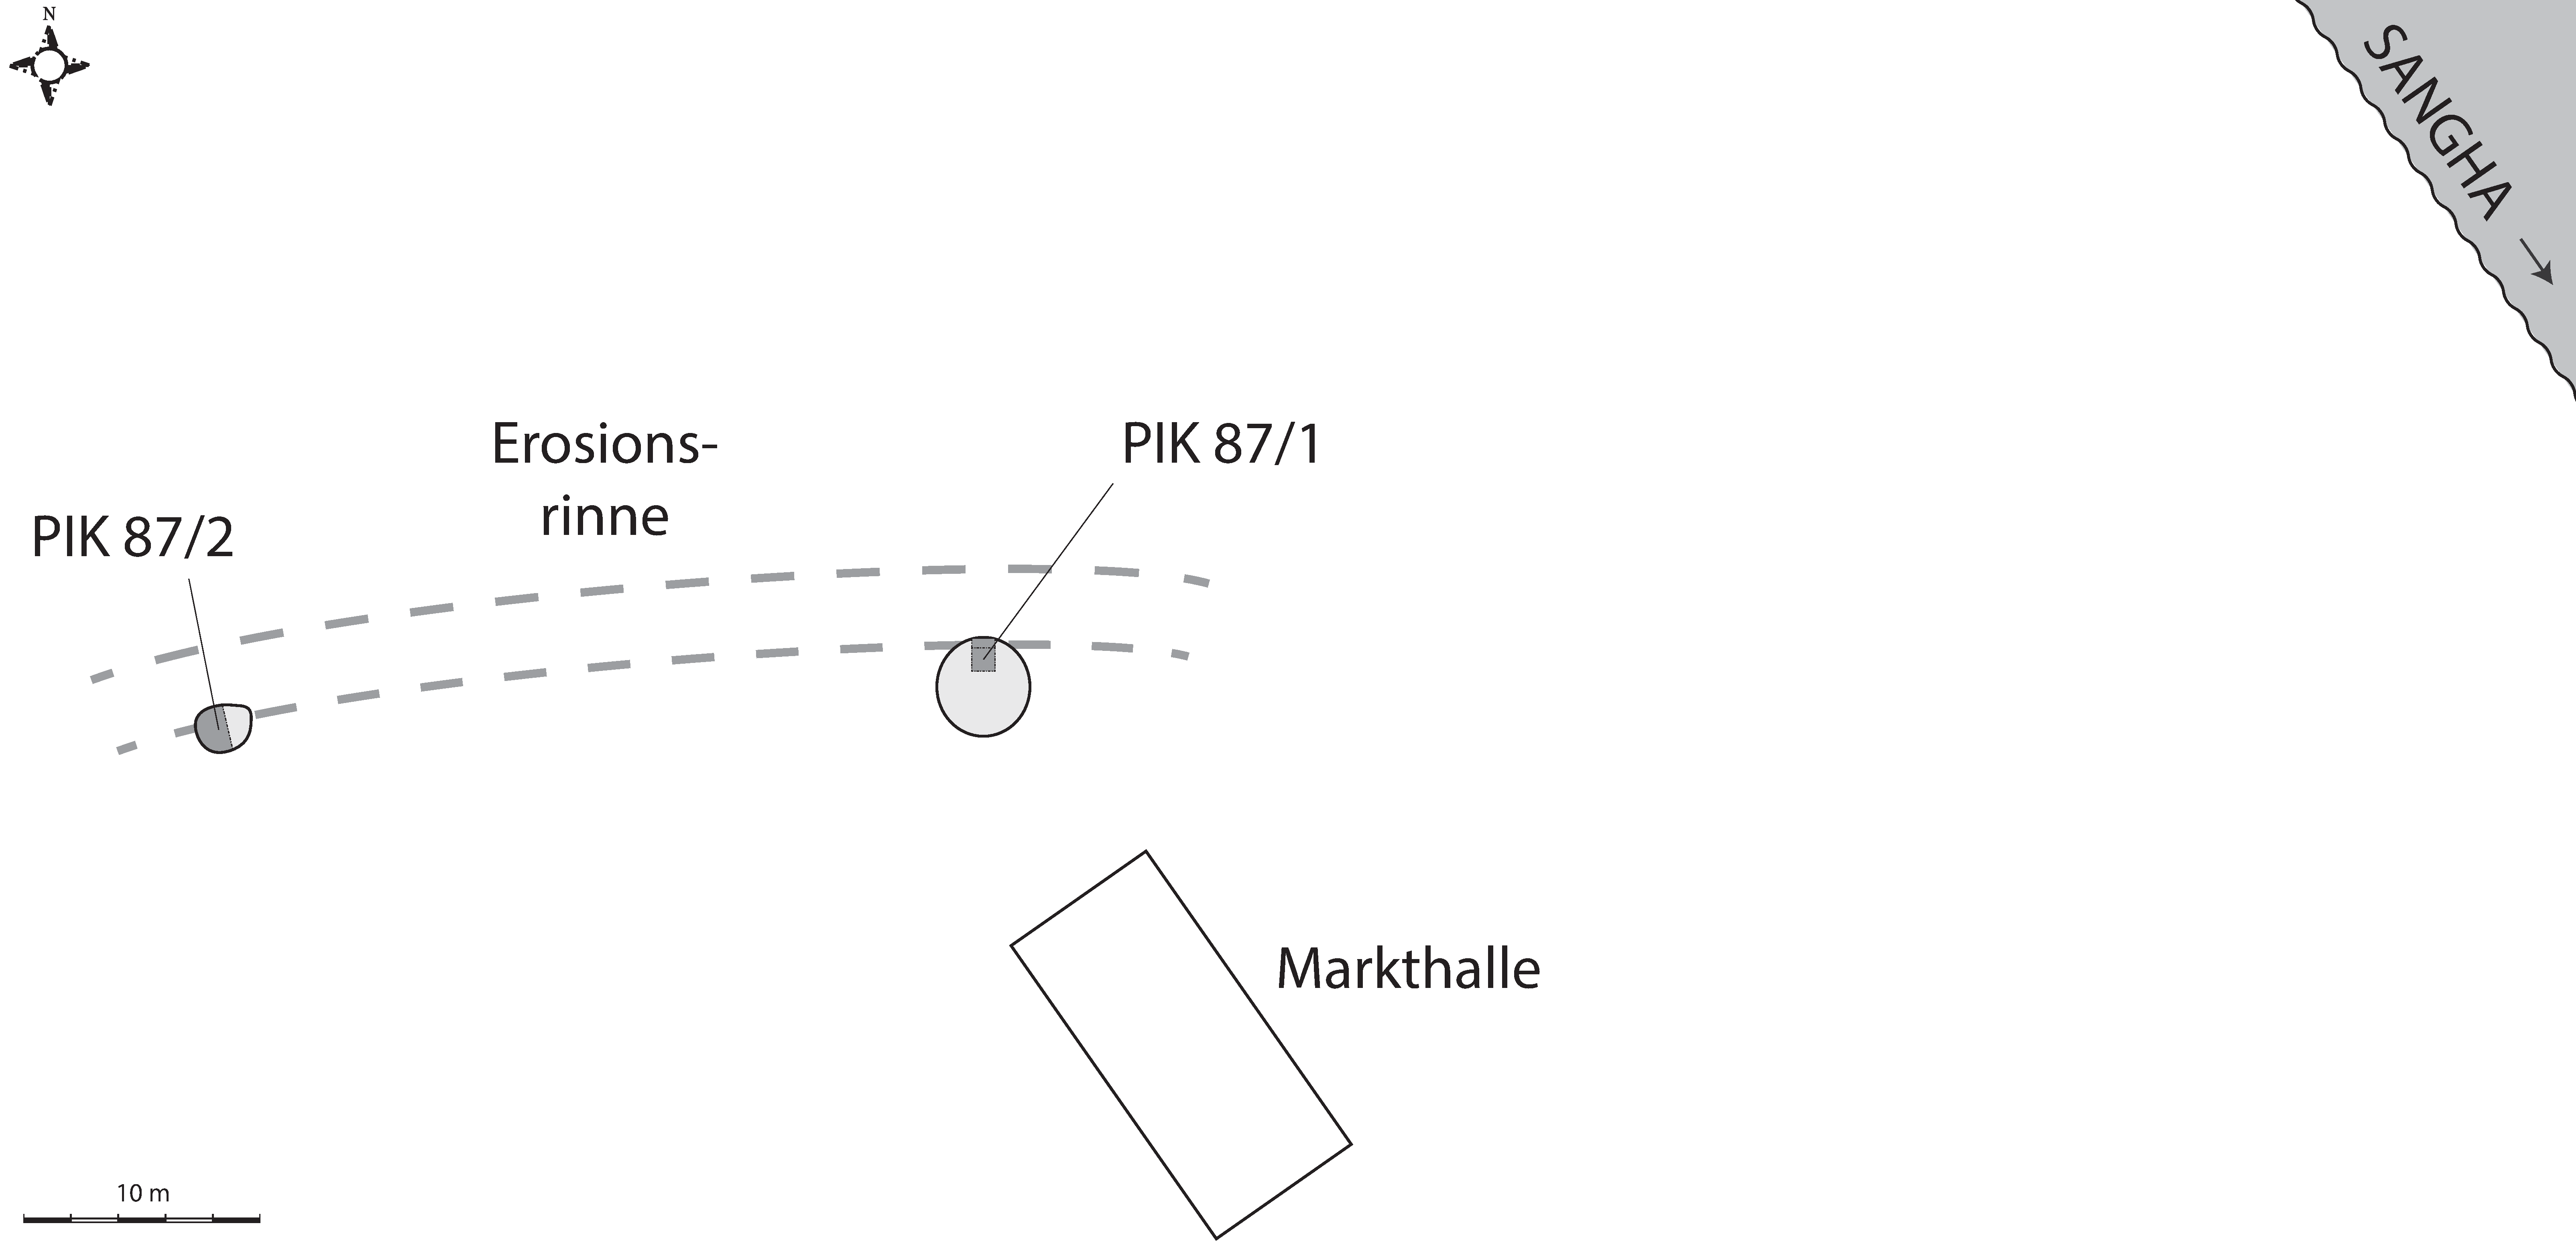
\includegraphics[width=\textwidth]{fig/PIK87_Uebersicht_2014-01-20.pdf}
 \caption{Pikunda (Fpl.~255): Grobe Lage der Grabungsstellen PIK~87/1 und PIK~87/2 (Kat.-Nr.~8--9; dunkelgrau: ausgegrabene Flächen).}
 \label{fig:PIK87_Fundstelle}
\end{figure*}

\begin{figure*}[!tb]
\centering
\begin{subfigure}[b]{\columnwidth}
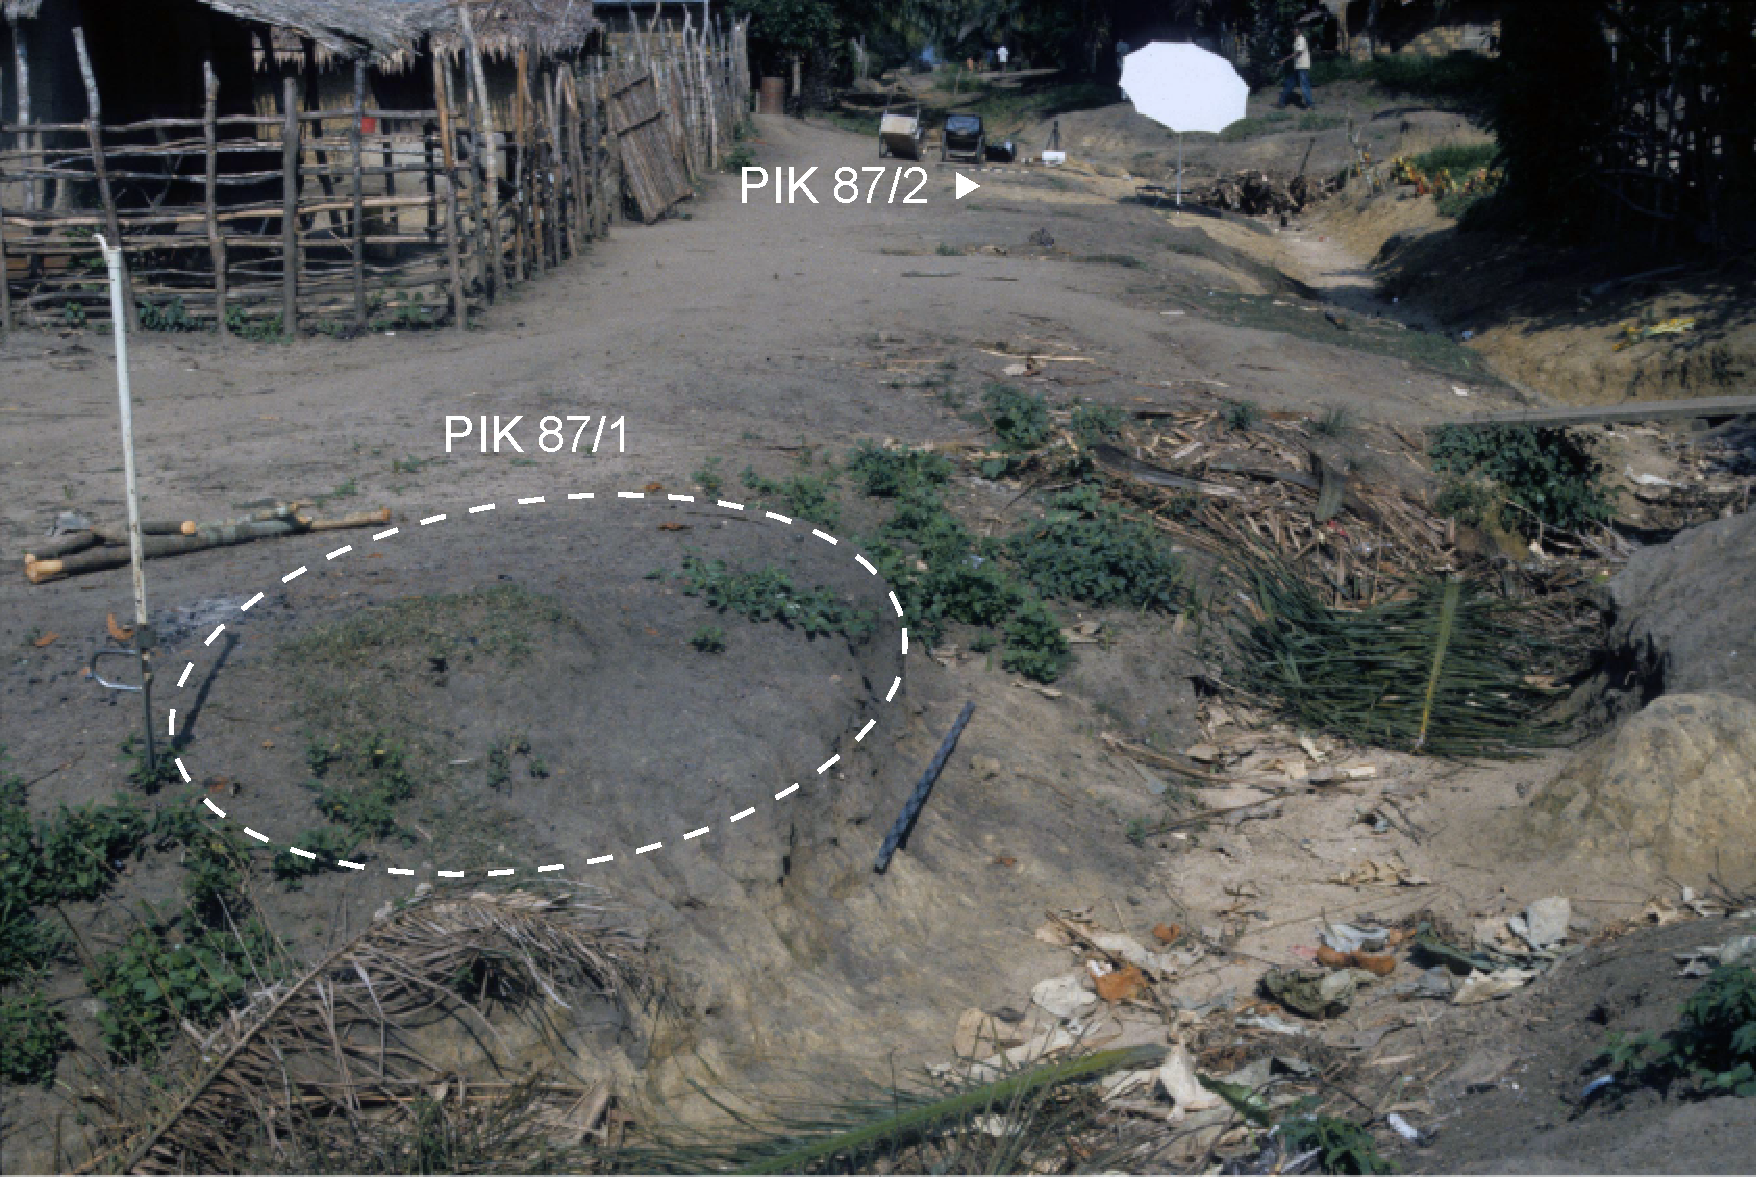
\includegraphics[width = \textwidth]{fig/PIK87-1_E87-014-6.pdf}
\caption{Übersicht von Nordwest.}
 \label{fig:PIK87-1_FundstelleObfl_vonNO}
\end{subfigure}\hfill
\begin{subfigure}[b]{\columnwidth}
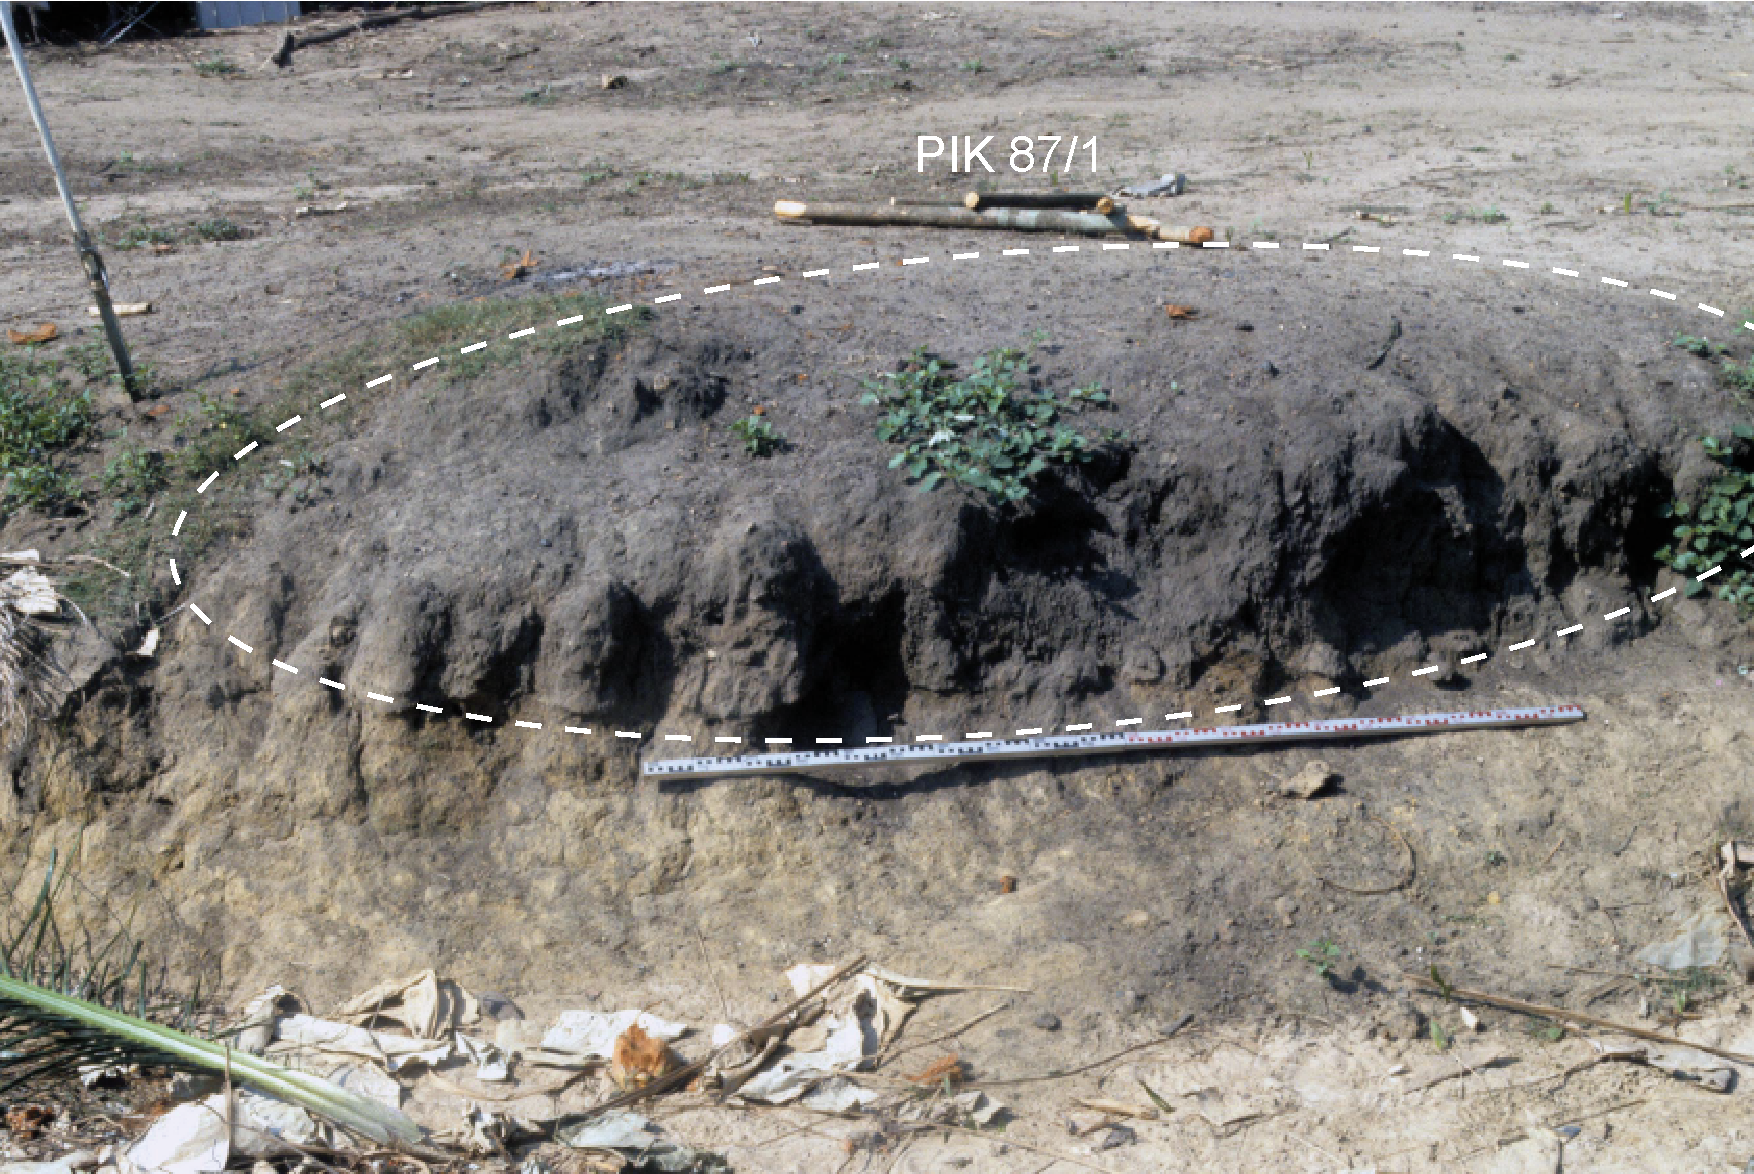
\includegraphics[width = \textwidth]{fig/PIK87-1_E87-014-3.pdf}
\caption{Blick von Nord.}
 \label{fig:PIK87-1_FundstelleObfl_vonN}
\end{subfigure}
 \caption{PIK~87/1: Grabungsstelle vor der Ausgrabung (Fotos: M. K. H. Eggert, 1987).}
 \label{fig:PIK87-1_FundstelleObfl_Foto}
\end{figure*}

\paragraph{Grabung und Befunde}\hspace{-.5em}|\hspace{.5em}%
In einer Erosionsrinne wurden bei einer ersten Prospektion am 12.\,05.\,1987 zwei teilweise freierodierte Gruben entdeckt (Kat.-Nr.~8--9). Im näheren Umfeld wurden drei Eisen-Verhüttungsöfen (\textsc{Kanimba Misago} 1995), von denen einer später unter der Kennung PIK~87/3 (Kat.-Nr.~10) untersucht wurde, und eine Reihe teilweise freierodierte Körperbestattungen gefunden. Neben Keramikscherben fand sich auch auffallend viel Eisenschlacke in diesem Bereich des Dorfes. Nach Abschluss der Prospektion entlang der Flüsse \mbox{Sangha} und \mbox{Ngoko} wurden die drei genannten Befunde systematisch ausgegraben. Die beiden Gruben liegen etwa 60\,m (PIK~87/1) beziehungsweise 90\,m (PIK~87/2) vom Ufer des \mbox{Sangha} entfernt (Abb.~\ref{fig:PIK87_Fundstelle}).\footnote{Die Lage des Verhüttungsplatzes PIK~87/3 (Kat.-Nr.~10) wurde weder beschrieben noch eingemessen und die Dokumentation des Ausgräbers C. Kanimba Misago liegt nicht vor.} Sie waren an der südlichen Kante einer nahezu Ost--West-verlaufenden, 4,5--5,5\,m breiten und 1,0--1,5\,m tiefen Rinne durch Erosion teilweise aufgeschlossen.

Die Grabungsstelle PIK~87/1 wurde zur Untersuchung einer etwa 4\,m großen, rundlichen, dunklen Verfärbung, die am östlichen Ende der Erosionsrinne beobachtet wurde, angelegt (Abb.~\ref{fig:PIK87_Fundstelle}, \ref{fig:PIK87-1_FundstelleObfl_Foto}).\footnote{Die Verfärbung war in O--W-Richtung 4\,m breit und vom Südende bis zum im Zuge der Grabung angelegten Nord-Profil waren es 3,8\,m (Abb.~\ref{fig:PIK87-1_PlanaSkizze}). Der Abstand zwischen dem Nord-Profil und der nördlichen Grubengrenze wurde nicht gemessen. Auf einigen Situationsfotos, die nach einem starken Regenschauer aufgenommen wurden, ist die Ausdehnung der dunklen Verfärbung deutlich zu sehen.} Die Grabung erfasste einen Teil des nördlichen Abschnitts dieser Verfärbung. Zu Beginn wurde ein etwa Ost--West-orientiertes, der Kante der Erosionsrinne folgendes Profil angelegt und der zügig abgetiefte Profilkasten als PIK~87/1/I bezeichnet (Abb.~\ref{fig:PIK87-1_PlanaSkizze}, \ref{fig:PIK87-1_ProfileFotos}).\footnote{Das bis auf etwa 3\,m unter die Oberfläche abgetiefte Profil diente vor allem der Bestimmung der Tiefe der die Verfärbung bildenden Befunde. Während des Aushebens des Profilkastens wurde nur wenig Keramik und kaum Holzkole gefunden. Teile eines Gefäßes fanden sich zwischen 1,65--1,75\,m unter der Oberfläche (Abb.~\ref{fig:PIK87-1_ProfileZeichnung}; Taf.~44.3). Weitere einzelne Scherben fanden sich zwischen 2,20--2,80\,m unter der Oberfläche. Erst ab etwa 2,80\,m, im Bereich der Sohle von Grube B1/B2, fand sich deutlich mehr Holzkohle sowie einige Brocken gebrannten Lehms.} Südlich an dieses Profil anschließend wurde eine 1\,$\times$\,1\,m große Fläche in 15 künstlichen, jeweils 20\,cm mächtigen Abträgen ausgegraben.\footnote{Eine Dokumentation von dabei angelegten Plana erfolgte nicht.} Durch die Grabung wurden zwei Gruben erfasst, die im Weiteren als Befund A und B bezeichnet werden. Die tiefere und ältere Grube B wird von einer jüngeren Grube A geschnitten (Abb.~\ref{fig:PIK87-1_ProfileZeichnung}, \ref{fig:PIK87-1_ProfileFotos}).\footnote{Obwohl während der Grabung keine Trennung des Fundmaterials aus diesen beiden Befunden erfolgte, lässt sich das Fundinventar eindeutig in zwei Komplexe unterteilen, die mit dem stratigrafischen Befund korrespondieren (Abb.~\ref{fig:PIK87-1_VerteilungStilgr}--D).}

\begin{figure*}[tb]
 \centering
 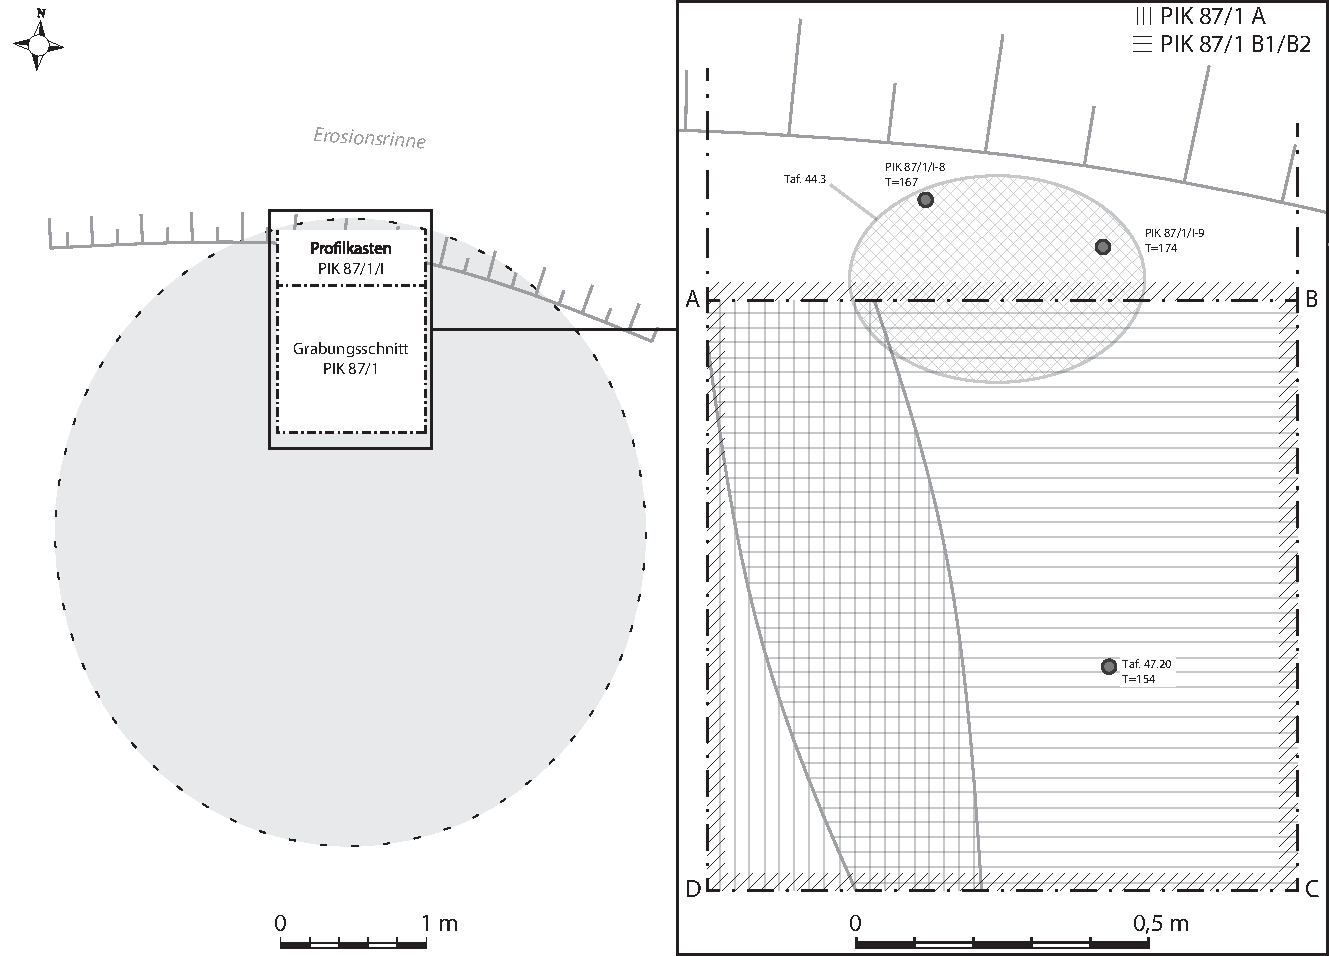
\includegraphics[width=\textwidth]{fig/PIK87-1_Planum_Keramik.pdf}
 \caption{PIK~87/1: Planskizze mit Positionsangaben zu eingemessenen Einzelfunden und summarische Rekonstruktion der Befundsituation im Planum (rechts).}
 \label{fig:PIK87-1_PlanaSkizze}
\end{figure*}

\begin{figure*}[p]
\centering
\begin{subfigure}[t]{\columnwidth}
 \centering
 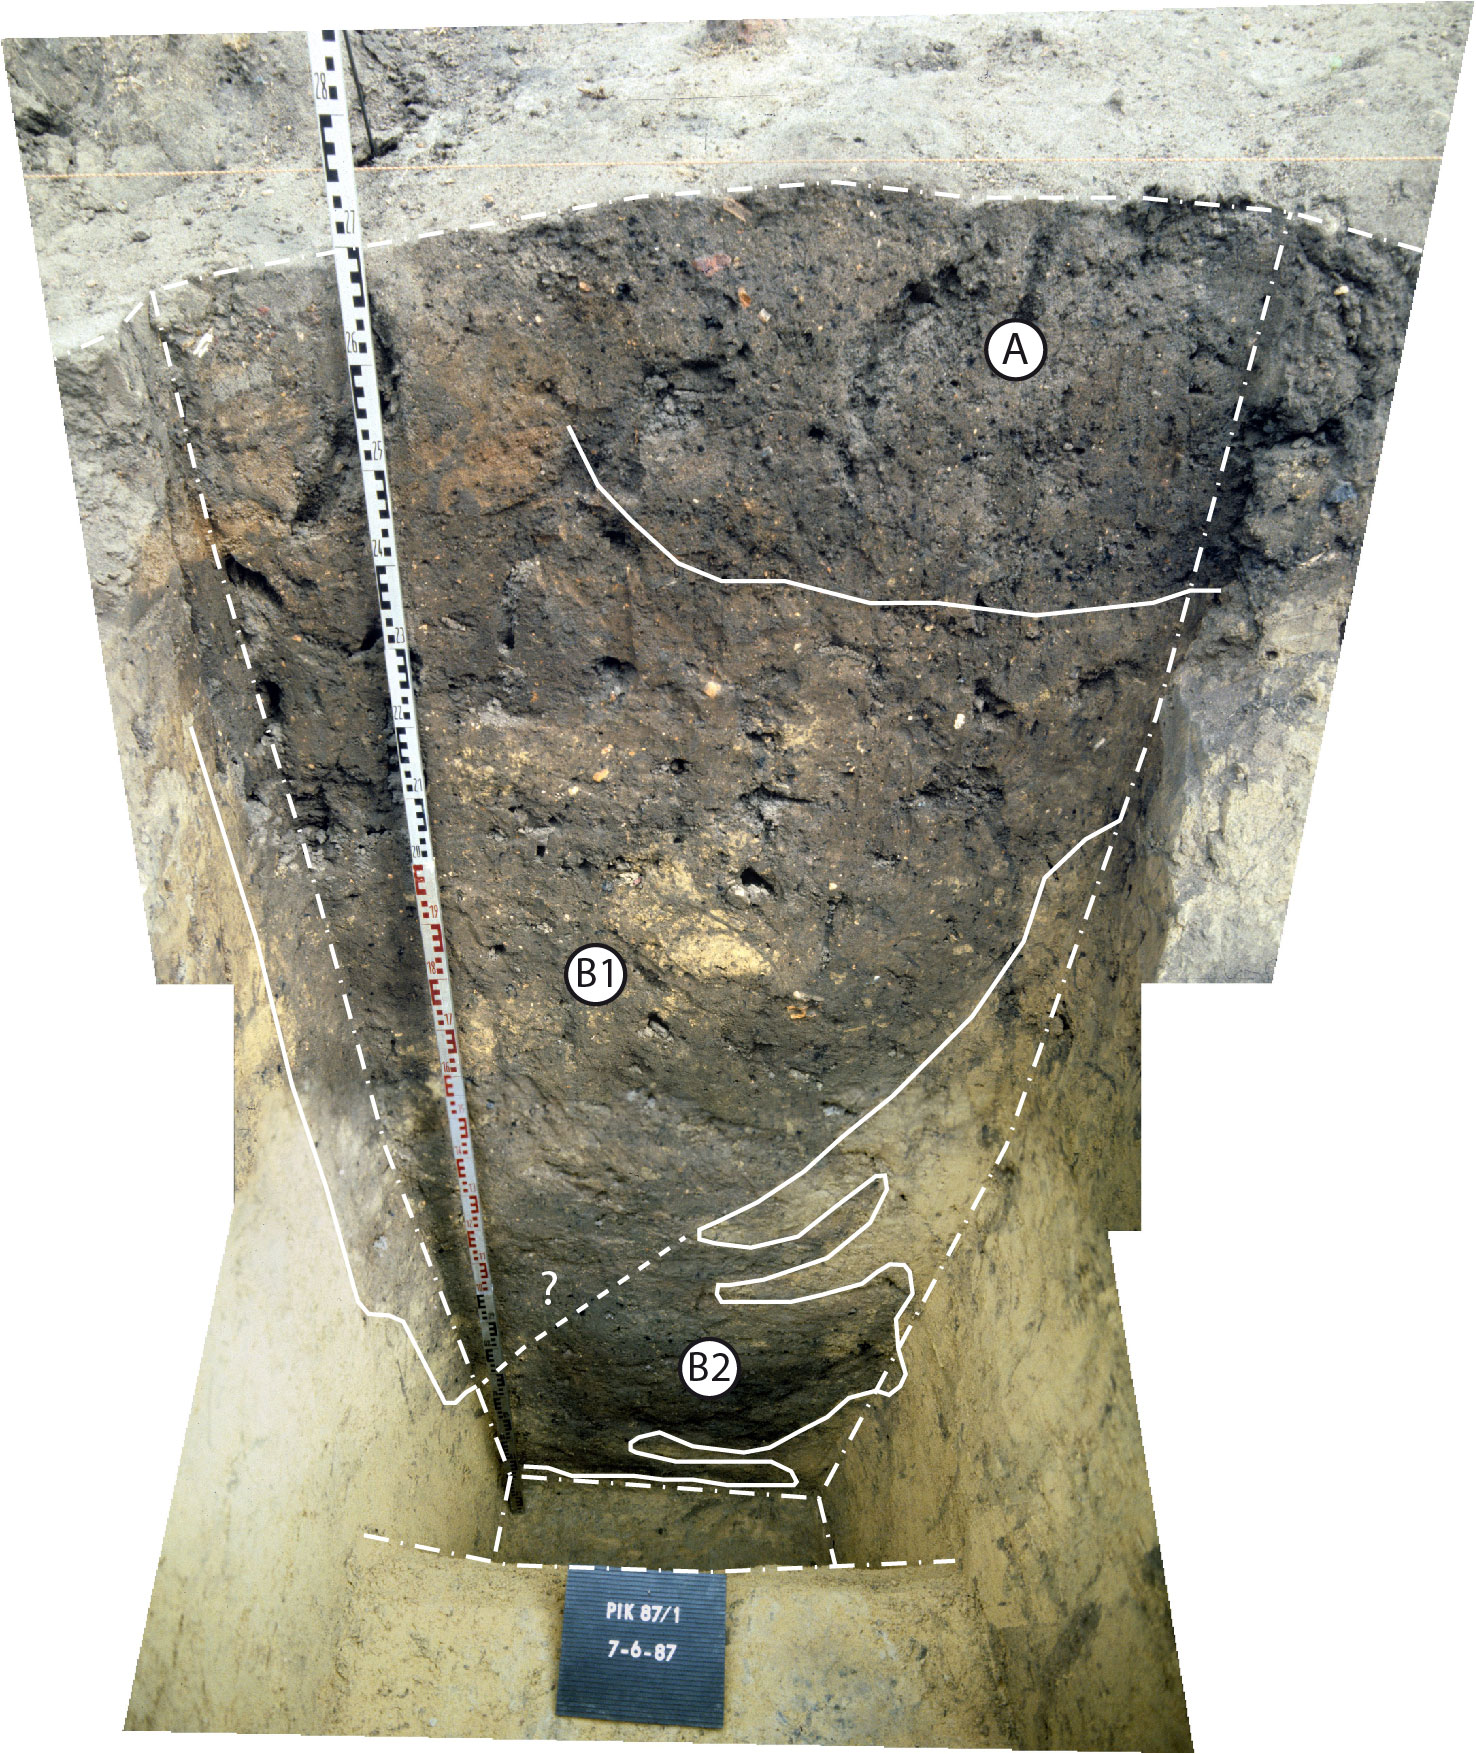
\includegraphics[width=\columnwidth]{fig/PIK87-1_N-profil_E87-018-26--28-01_2014-01-01.jpg}
 \caption{Nord-Profil}
 \label{fig:PIK87-1_N-Prof}
\end{subfigure}\hfill
\begin{subfigure}[t]{\columnwidth}	
 \centering
 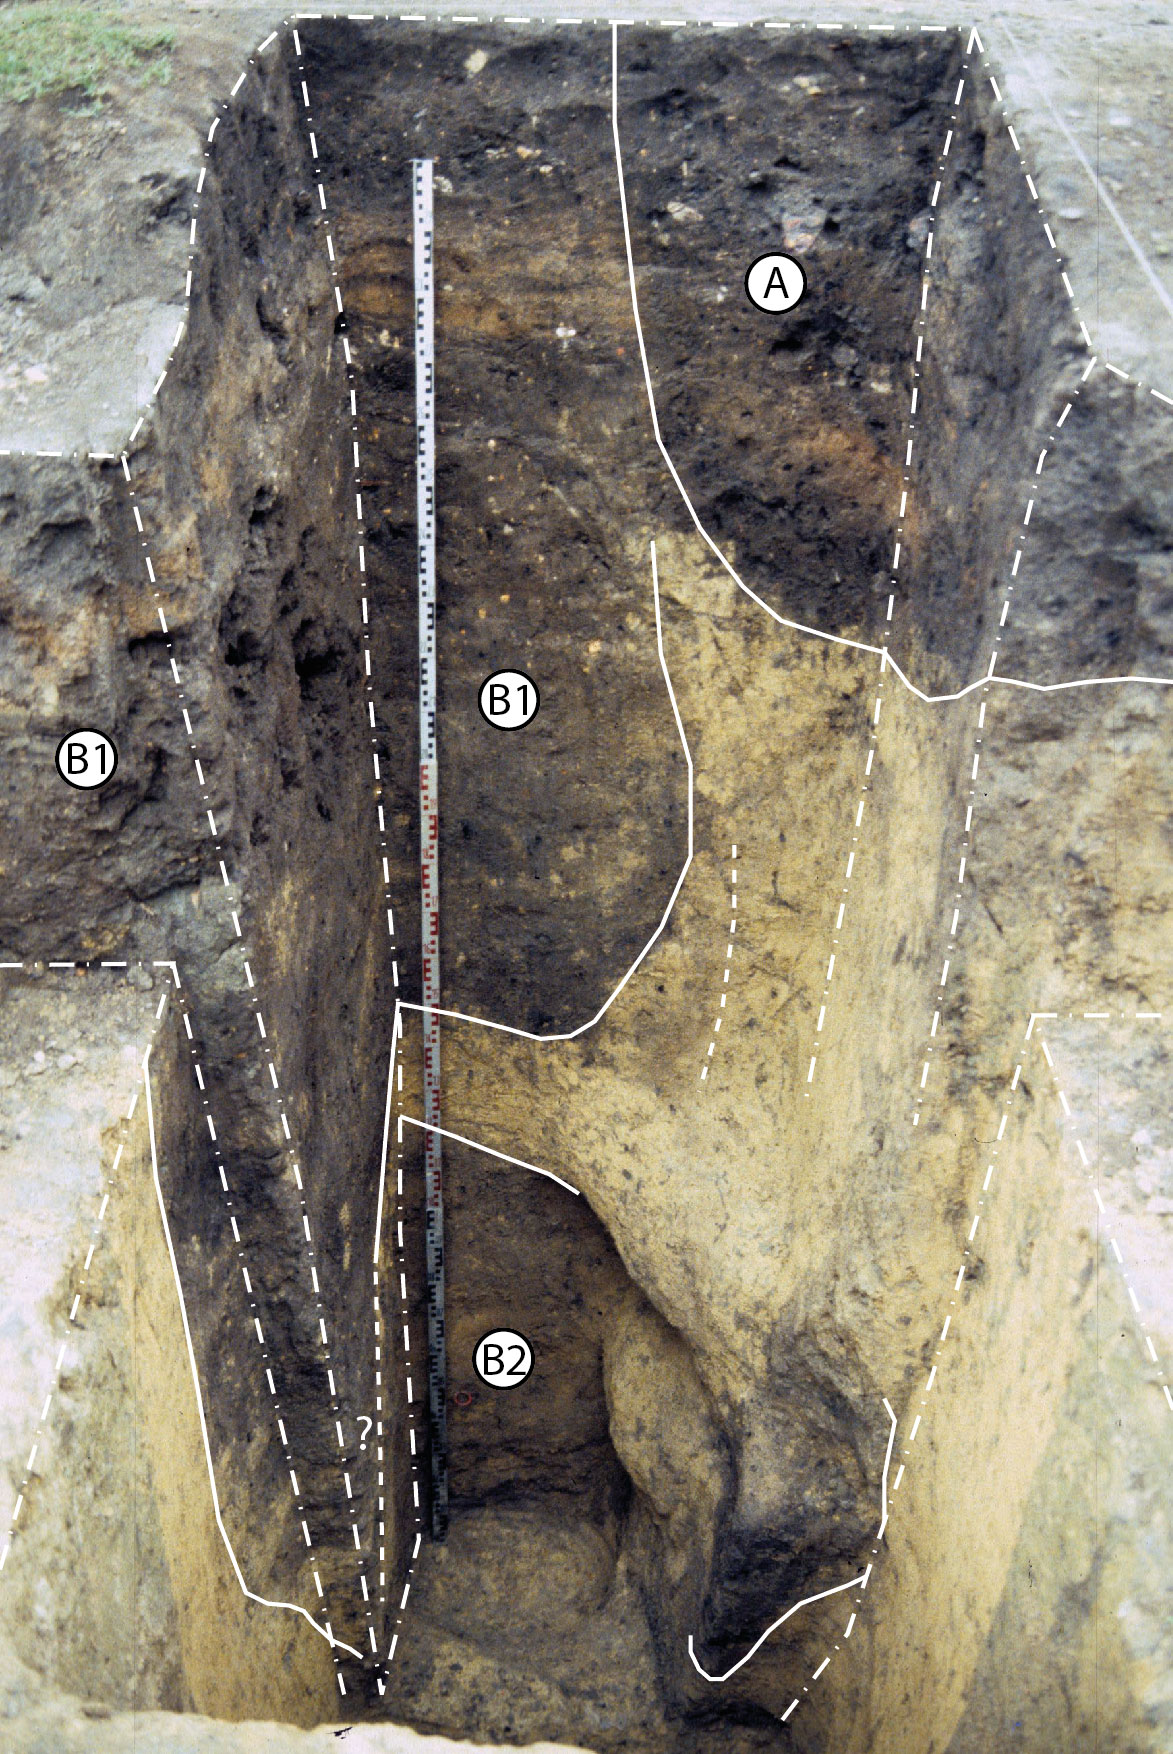
\includegraphics[width=.8\columnwidth]{fig/PIK87-1_S-Profil_E87-020-2_2014-01-01.jpg}
 \caption{Grabungsschnitt mit Ost-, Süd- und West-Profil}
 \label{fig:PIK87-1_O+S+W-Prof}
\end{subfigure}
 \caption{PIK~87/1: Profile (Fotos: M.~K.~H. Eggert, 1987).}
 \label{fig:PIK87-1_ProfileFotos}
\end{figure*}

\begin{figure*}[p]
	\centering
	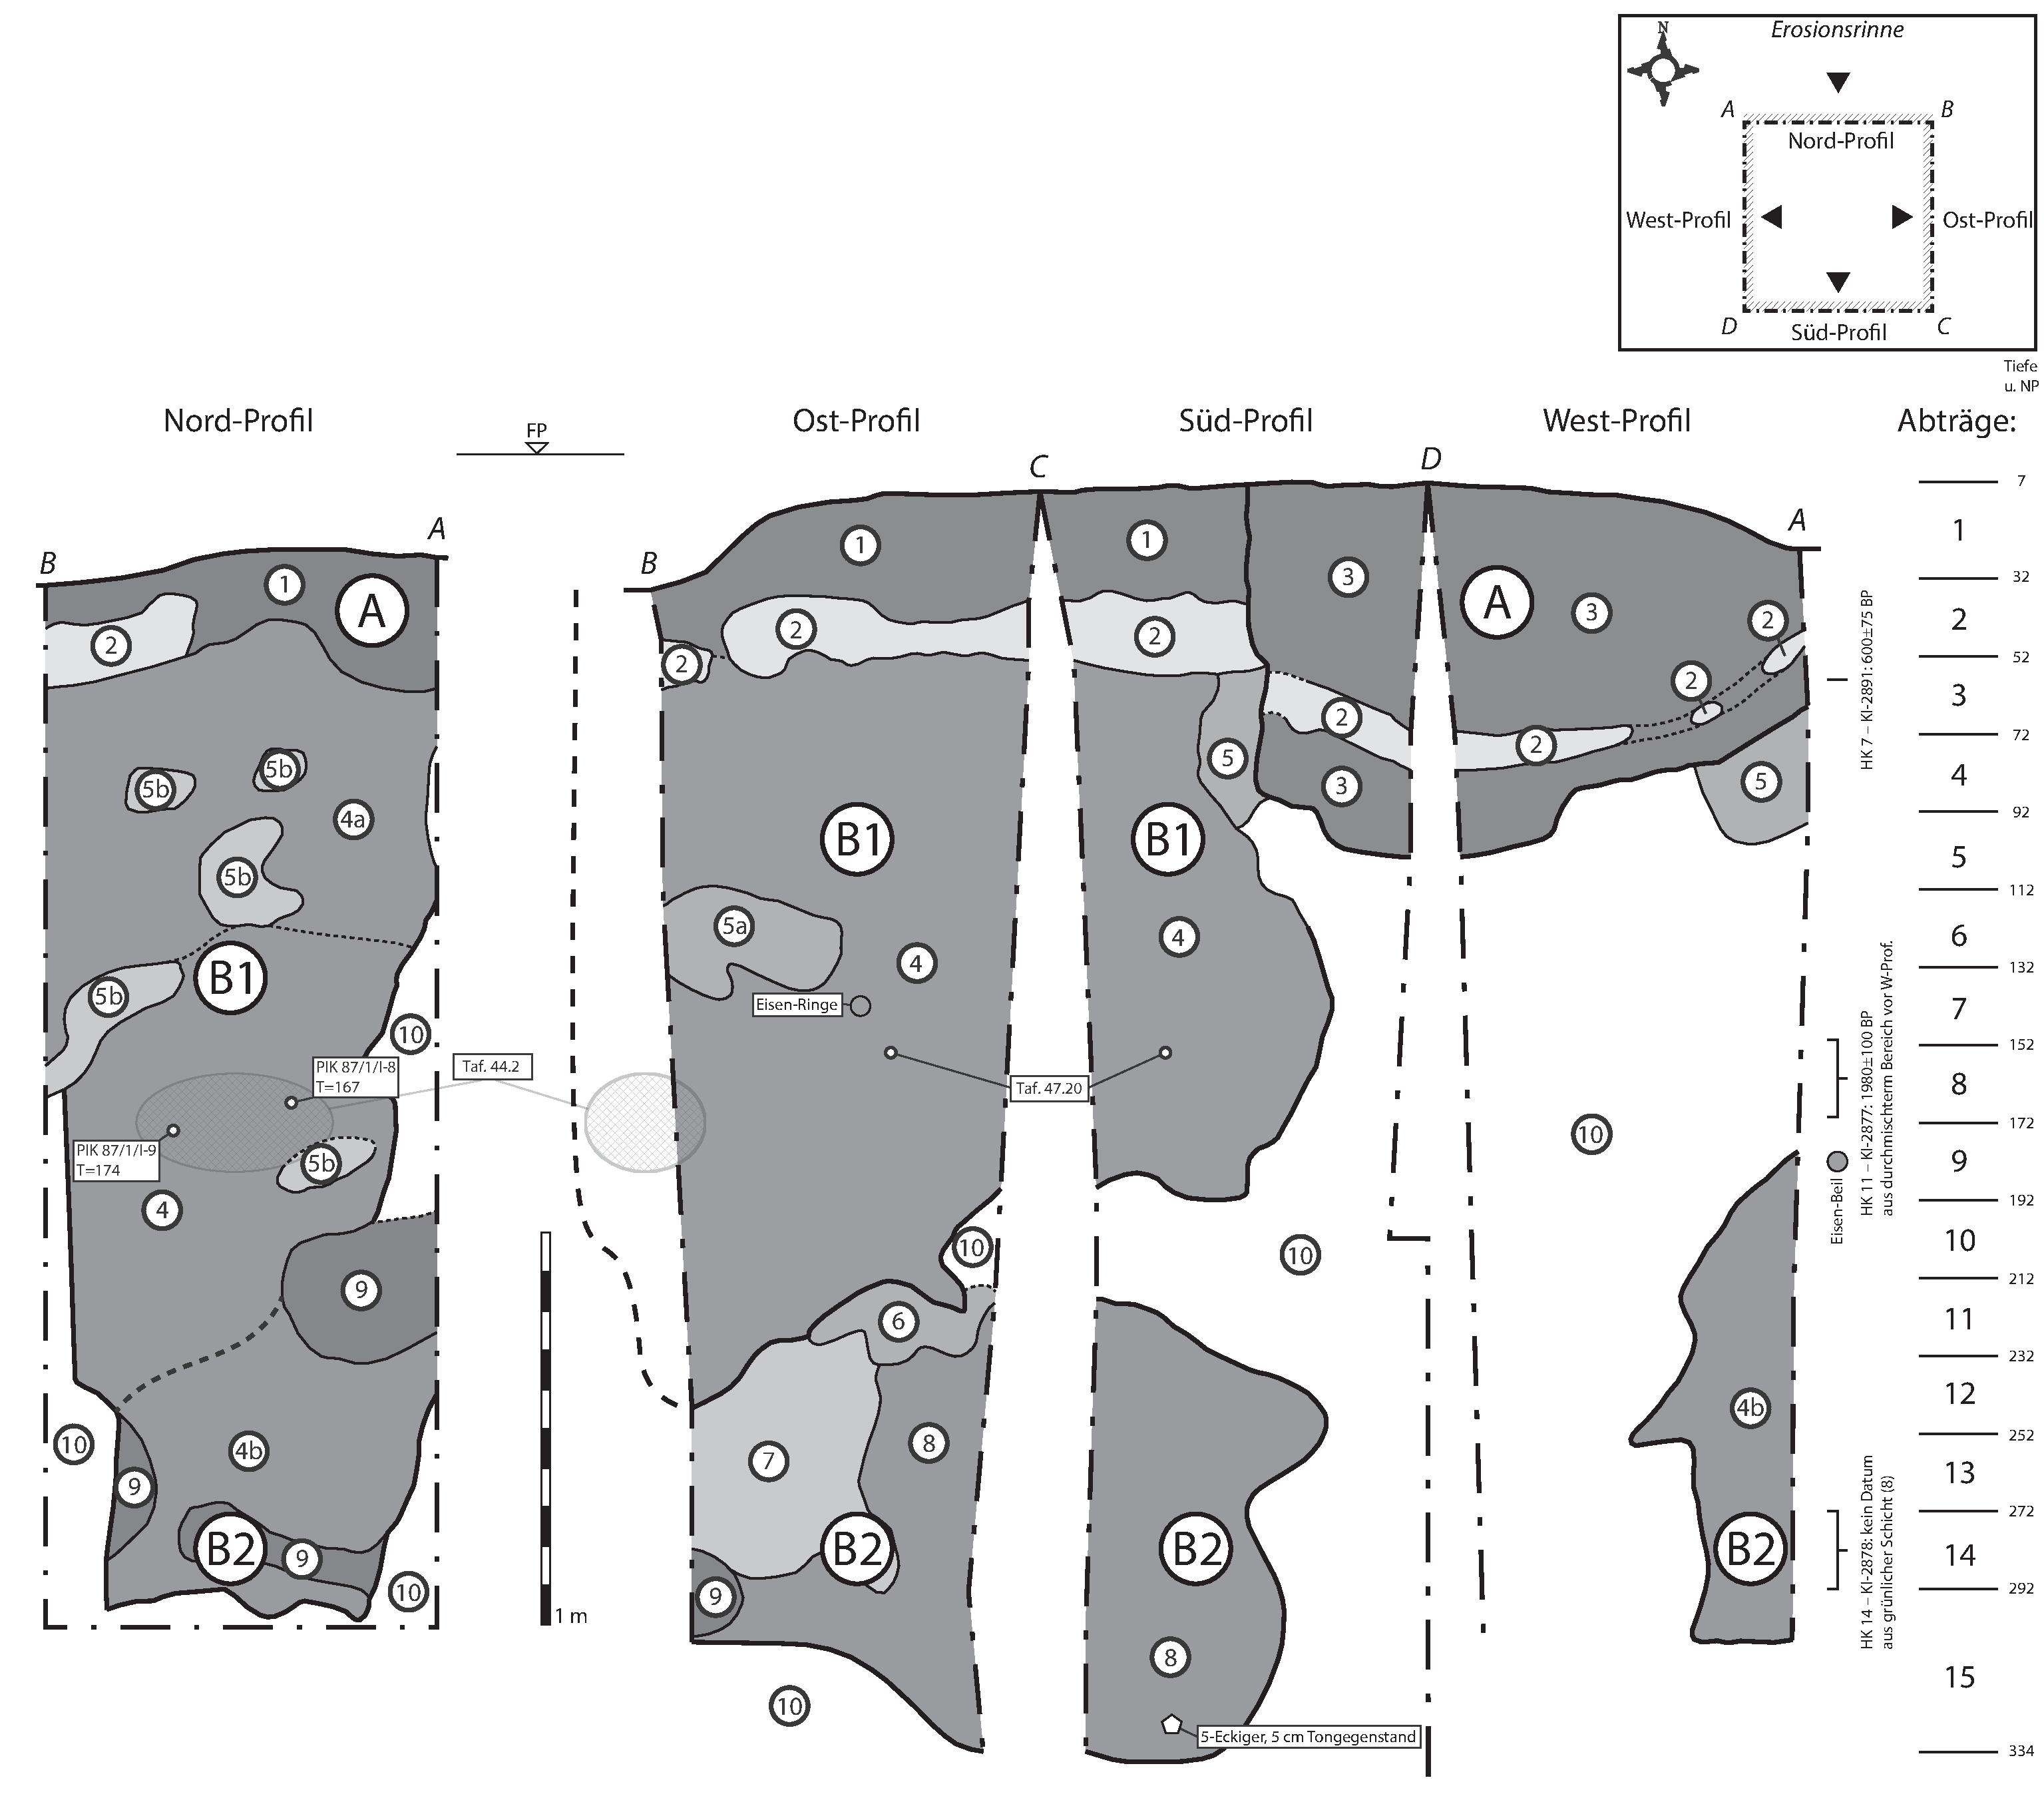
\includegraphics[width=.9\textwidth]{fig/PIK87-1.pdf}
	\caption{PIK~87/1: Profile.}
	\label{fig:PIK87-1_ProfileZeichnung}
\end{figure*}

Die bis 0,95\,m unter die heutige Oberfläche reichende Grube A wurde im südwestlichen und westlichen Teil des Schnittes erfasst (Abb.~\ref{fig:PIK87-1_ProfileZeichnung}). Der Befund greift in den oberen Bereich der Grube B1/B2 ein und ist folglich stratigrafisch jünger (Abb.~\ref{fig:PIK87-1_ProfileFotos}). Die Wandung von Grube A ist vertikal bis steilschräg, ihre Sohle konvex und die Ecken gerundet bis fließend. Da die Begrenzung des Befundes lediglich im Süd-Profil erfasst wurde, können keine sicheren Angaben zum Durchmesser der Grube gemacht werden (Abb.~\ref{fig:PIK87-1_ProfileZeichnung}).\footnote{Der bei der Grabung erfasste Teil von Grube A entspricht grob einem Volumen von 0,3\,m\textsuperscript{3}. Im Westprofil war die nördliche Grenze der Grube bereits durch Erosion abgetragen. Unter der Annahme, dass in nördlicher Richtung ein eher fließenderer Übergang von Sohle und Wandung vorlag und die bei Profilnagel D erfasste Tiefe der tiefste Punkt des Befundes ist, würde die nördliche Begrenzung etwa 30--40\,cm über die Erosionsrinne hinausragen. Auf Basis dieser Annahmen und dem Schnittpunkt der Grube im Westprofil ließe sich ein Durchmesser von etwa 2,6\,m rekonstruieren. Mit einem solchen Durchmesser würde eine runde Grube allerdings 0,5--1,0\,m über die maximale Ausdehnung der an der Oberfläche sichtbaren Verfärbung hinausreichen. Eventuell ist daher mit einer eher ovalen Form der Grube A zu rechnen.} Auffällig ist die rötliche Schicht~2, die etwa 0,3--0,4\,m unterhalb der rezenten Oberfläche horizontal durch beide Befunde verläuft. In Grube A ist diese Schicht allerdings um etwa 0,2--0,3\,m nach unten versetzt und befindet sie sich in einer Tiefe von etwa 0,5--0,7\,m unter der Oberfläche (Abb.~\ref{fig:PIK87-1_ProfileZeichnung}).\footnote{Ob es sich bei dem Material der Schicht 2 um einen Teil des Aushubs handelt, der später wieder mit verfüllt wurde, muss offenbleiben, kann aber als wahrscheinlich angenommen werden.}

Die stratigraphisch ältere Grube B lässt sich in zwei Bereiche untergliedern. Der obere Teil B1 reicht bis mindestens 2,7\,m unter die heutige Oberfläche. Die Verfüll-Schichten~4 und 4a sind homogen mittel- bis dunkelbraun und weisen teilweise hellere Einschlüsse auf, die Schichten~5a und 5b. Im Südprofil wurde die vertikale bis leicht konvexe Grubenwandung bis zu einer Tiefe von etwa 1,8\,m unter der heutigen Oberfläche, beziehungsweise 0,9\,m oberhalb der Sohle des unteren Bereichs B2 erfasst. Die Unterkante des Abschnitts B1 fällt schräg, mit etwa 30$^\circ$ Neigung nach Nordosten ab. Der tiefste erfasste Punkt dieses oberen Bereiches liegt im Bereich von Nagel B (Abb.~\ref{fig:PIK87-1_PlanaSkizze}, \ref{fig:PIK87-1_O+S+W-Prof}, \ref{fig:PIK87-1_ProfileZeichnung}).\footnote{Die nördliche Grubenwandung liegt etwa 0,2--0,3\,m nördlich des Nord-Profils (Abb.~\ref{fig:PIK87-1_O+S+W-Prof}, \ref{fig:PIK87-1_ProfileFotos}, \ref{fig:PIK87-1_ProfileZeichnung}).} Unterhalb des Verfüllpaketes B1 befindet sich ein weiteres, B2 genanntes Paket, das im westlichen Bereich teilweise vom anstehenden Lehm (Schicht 10) überlagert wird. Die Verfüllung dieses Bereiches (Schichten~4b und 6--9) ist heterogener als der obere Teil B1. Es sind deutlich häufiger gelbe, lehmige Linsen beziehungsweise Einschlüsse zu beobachten und grundsätzlich ist das Substrat etwa heller, als das des oberen Bereiches. Schicht~8 wird zudem als leicht grünlich beschrieben. Sie enthielt den Großteil, der nur noch eher spärlichen Keramik aus diesem Abschnitt. An der Sohle fanden sich keine bis kaum Funde, aber weiterhin sehr viel Holzkohle. Der Grubenteil B2 wurde bis etwa 3,25\,m unter die heutige Oberfläche nachvollzogen. Ab dieser Tiefe fanden sich kleine Laterit-Knollen.

%\vspace{1.5em}
\columnbreak
\noindent Die Grabung erbrachte den folgenden stratigrafischen Befund (Abb.~\ref{fig:PIK87-1_ProfileZeichnung}):
\begin{itemize}[leftmargin=*, labelindent=1.25em, noitemsep, topsep=0pt]
\item [(1)] 10 YR 3/1 bis 10 YR 3/1.5; Sand (S)
\item [(2)] 10 YR 4.5/5; Sand (S) mit dunklerem Boden (etwa 2.5 Y 3/2)
\item [(3)] 10 YR 3/2; toniger Sand (tS); mehr Holzkohle als in den anderen Schichten
\item [(4)] 10 YR 3.5/3; toniger Lehm (tL)
\item [(4a)] 10 YR 3/2; toniger Lehm (tL)
\item [(4b)] 10 YR 3.5/2; toniger Lehm (tL)
\item [(5)] 10 YR 3/3; schluffiger Lehm (uL); heterogen gelblich
\item [(5a)] 10 YR 3/3 mit 10 YR 6/5; sandiger Ton (sT)
\item [(5b)] 10 YR 4/3; durchmischt mit 10 YR 6/6, lehmig
\item [(6)] 10 YR 3/3; schluffiger Lehm (uL)
\item [(7)] 10 YR 6/3.5 bis 2.5 Y 6/3; toniger Lehm (tL)
\item [(8)] 2.5 Y 4/2; grünlich; lehmiger Schluff (lU); teils auch etwas mit Gelb durchmischt
\item [(9)] 2.5Y 4/4 bis 10 YR 3.5/3 bis 10 YR 6/6; toniger Lehm (tL)
\item [(10)] 10 YR 6/6; toniger Lehm (tL)
\end{itemize}

\begin{table*}[tb]
	\vspace{2em}
	\centering
	%{\footnotesize \begin{sftabular}{@{}p{.1\textwidth}p{.1\textwidth}p{.15\textwidth}p{.15\textwidth}p{.4\textwidth}@{}}
	{\footnotesize \begin{sftabular}{@{}lllrll@{}}\toprule 
			\textbf{Grube} & \textbf{Bereich} & \textbf{Abträge} & \textbf{Tiefe} & \textbf{Schichten} & \textbf{keramische Stilgruppen} \\ 
			\midrule 
			A & & 1--5 & 0--1,03\,m & 3 & Mandombe (Ebambe, Matoto, Konda, Pandama, Mbenja) \\ 
			\multirow{2}{*}{B} & 1 & 1--12 & 0--2,34\,m & 4, 4a, 5a, 5b & Pikunda-Munda (\mbox{Ngbanja} und evtl. Lusako) \\ 
			& 2 & 9--15 & 2,10--3,36\,m & 4b, 6, 7, 8, 9 & Pikunda-Munda (evtl. Lusako) \\ 
			\bottomrule 
	\end{sftabular}}
	\caption{PIK~87/1: Erfasste Gruben.}
	\label{tab:PIK87-1_Befunde}
\end{table*}

\begin{table*}[tb]
	\centering
	{\footnotesize \begin{sftabular}{@{}lrrrr@{}}
\toprule
   \textbf{Fundkategorie} &  \textbf{Anzahl} &    \textbf{\%} &  \textbf{Gewicht (kg)} &    \textbf{\%} \\
\midrule
           Eisen &       3 &   0,4 &          0,06 &   0,2 \\
 gebrannter Lehm &       9 &   1,3 &          0,09 &   0,3 \\
         Keramik &     462 &  67,3 &         23,28 &  79,9 \\
         Knochen &       9 &   1,3 &          0,25 &   0,9 \\
        Ofenwand &       4 &   0,6 &          0,03 &   0,1 \\
        Schlacke &     162 &  23,6 &          4,88 &  16,7 \\
          Sonder &       3 &   0,4 &          0,01 &   0,0 \\
           Stein &      32 &   4,7 &          0,53 &   1,8 \\
          Tuyère &       2 &   0,3 &          0,01 &   0,0 \\
\bottomrule
\end{sftabular}
}
	\caption{PIK~87/1: Anteil verschiedener Fundmaterialien.}
	\label{tab:PIK87-1_Funde}
\end{table*}

\paragraph{Keramik\vspace{.5em}}\mbox{}\\
\begin{tabular}{@{}lrl@{}}
	Ausgesondert: & 11\,300\,g & \textit{40\,\% glatte Wandung} \\
	& & \textit{60\,\% rauwandig} \\
	Ausgezählt: & 2886\,g & \\
	Bearbeitet: & 9137\,g & (76\,\%) \textit{ohne 1987} \\
	& & \textit{ausgesondertes Material} \\
	Insgesamt: & 23\,323\,g &
\end{tabular}

\vspace{1em}
\noindent 
Die durch die Grabung erfassten Funde zeichnet die geschilderte Befundsituation und Unterschiede der beiden erfassten Gruben nach (Abb.~\ref{fig:PIK87-1_VerteilungFunde}). Das Gros -- zirka 78\,\% -- aller Funde fand sich in den hauptsächlich mit der Grube A zu assoziierenden, obersten vier Abträgen.\footnote{Im Zuge der Reinigung und Durchsicht der Funde am Ende der Feldkampagne von 1987 wurden im Materiallager in Bamanya etwa 50\,\% der aus der Grabung PIK~87/1 stammenden Keramik als \textit{nicht diagnostisch} ausgesondert. Die Stücke wurden in \textit{glatt}- und \textit{rau}-wandig unterschieden und nach Abträgen getrennt summarisch gewogen. Einige Scherben der beiden Gruppen wurden stellvertretend mitgenommen. Bei den Referenz-Scherben der \textit{rau}-wandigen Keramik handelt es sich durchweg um mit Schlickerrauung versehene Scherben des Mandombe-Stils (Kap.~\ref{sec:MDB-Gr}). Schlickerrauung lässt sich im untersuchten Material nur auf den unteren Hälften von Gefäßen dieser Stilgruppe beobachten. Die 1987 ausgesonderte, \textit{rau}-wandige Keramik kann unter Vorbehalt der Mandombe-Gruppe zugeordnet werden. Unter den Referenzstücken der \textit{glatt}-wandigen Keramik sind neben Stücken, die -- aufgrund ihres Scherbens (\textit{Fabric}~1) -- der Pikunda-Munda-Gruppe zugerechnet werden können, auch solche, die der Mandombe-Gruppe (\textit{Fabric}~3) zuzurechnen sind. Da oberhalb des fünften Abtrages (T~112) keramisches Material der Stilgruppen Mandombe (Grube A) und Pikunda-Munda (Grube B1) gemeinsam auftreten, ist eine Integration der 1987 ausgesonderten \textit{glatt}-wandigen Keramik oberhalb von etwa 1\,m Tiefe nicht mehr möglich. Die unterhalb dieser Tiefe ausgesonderte, \textit{glatt}-wandige Keramik kann, von vereinzelten Importstücken abgesehen, grundsätzlich nur der Pikunda-Munda-Gruppe (Kap.~\ref{sec:PKM-Gr}) zugerechnet werden. Im Material finden sich keine Scherben der Mandombe-Gruppe unterhalb des fünften Abtrages. Auffällig ist, das sich in den Abträgen 7--8 (T~152--172) auch knapp 200\,g \textit{rau}-wandige Keramik fanden. Es ist anzunehmen, das es sich dabei nicht um schlickergeraute Scherben der Mandombe-Gruppe gehandelt hat, sondern um \textit{gröbere} Keramik der \mbox{Ngbanja}-Gruppe (Kap.~\ref{sec:NGB-Gr}). Vertreter der \mbox{Ngbanja}-Gruppe finden sich in dieser Tiefe auch im aufgenommen Material (Abb.~\ref{tab:PIK87-1bis9_nichtPIK-MUN}).} Unterhalb dieses Bereiches steigt das Fundaufkommen in den Abträgen 8--9, etwa 1,8\,m unter der heutigen Oberfläche, noch einmal leicht an.\footnote{Der Anstieg des Fundaufkommens bei etwa 1,8\,m unter der Oberfläche (Abb.~\ref{fig:PIK87-1_VerteilungFunde}) ist vor allem einem fast vollständigen Gefäß (Taf.~44.3) sowie einem großen Gefäßfragment (Taf.~45.2) geschuldet.} Nichtkeramische Funde machen etwa 20\,\% des gesamten Fundgutes aus und finden sich verstärkt in den auch an Keramik reichen Abträgen.

\begin{figure*}[p]
	\centering
	\begin{subfigure}{\textwidth}	
		\centering
		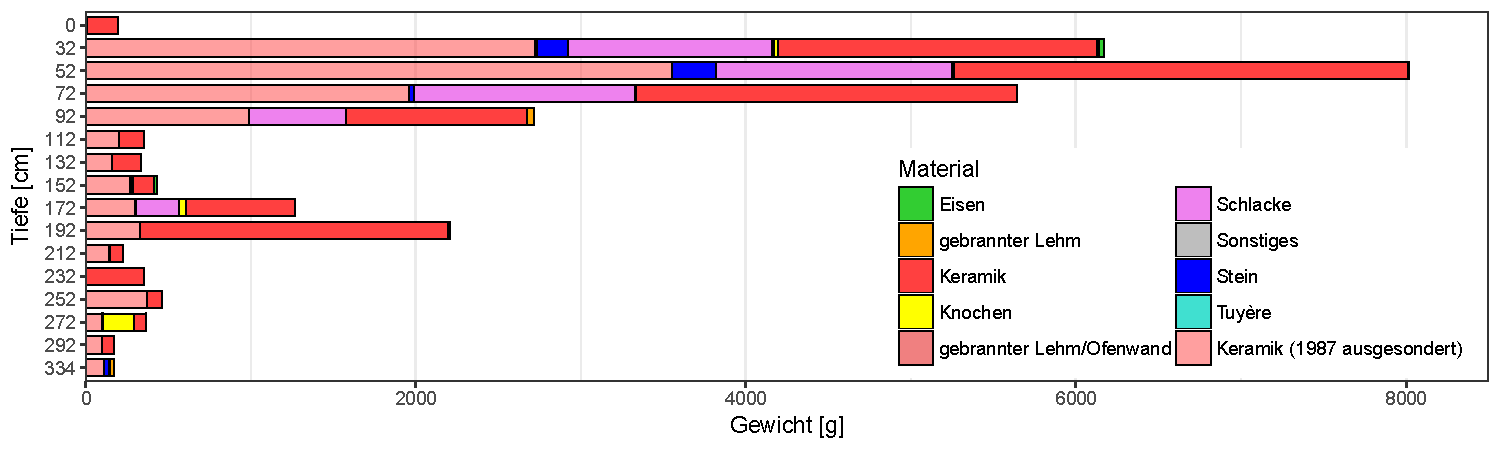
\includegraphics[width = \textwidth]{fig/9-8_PIK87-1_VerteilungFunde_R.pdf}
		\caption{Fundmaterial.\vspace{1em}}	
		\label{fig:PIK87-1_VerteilungFunde}
	\end{subfigure}
	\begin{subfigure}{\textwidth}
		\centering
		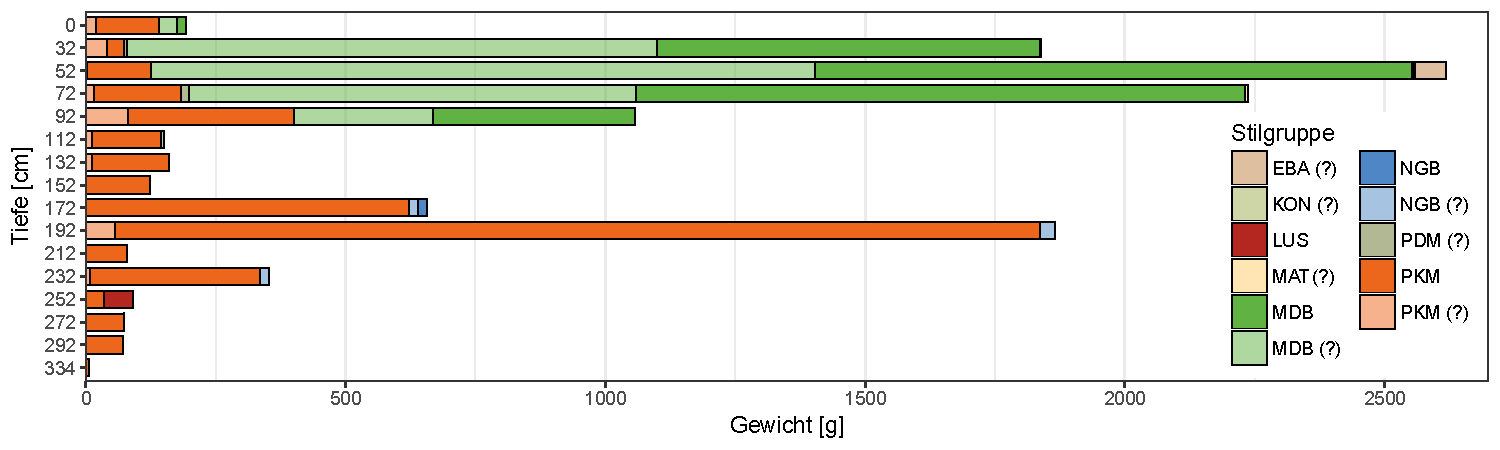
\includegraphics[width = \textwidth]{fig/9-8_PIK87-1_KeramikStilgruppen_R.pdf}
		\caption{Keramische Stilgruppen.\vspace{1em}}
		\label{fig:PIK87-1_VerteilungStilgr}
	\end{subfigure}
	\begin{subfigure}{\textwidth}	
		\centering
		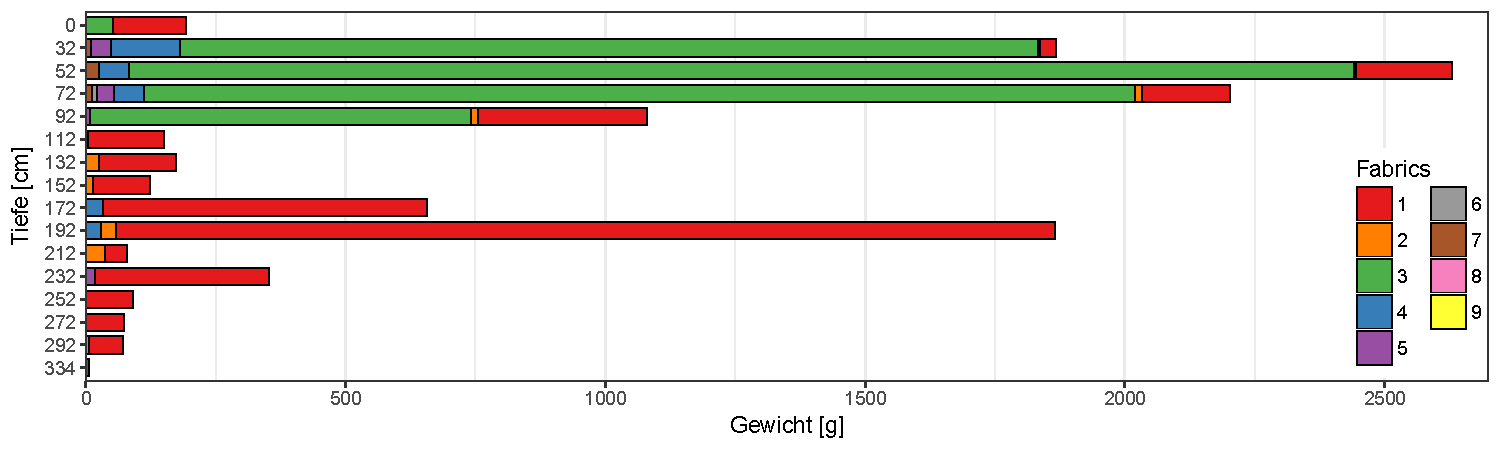
\includegraphics[width = \textwidth]{fig/9-8_PIK87-1_Fabrics_R.pdf}
		\caption{\textit{Fabrics}.\vspace{1em}}
		\label{fig:PIK87-1_VerteilungFabrics}
	\end{subfigure}
	\begin{subfigure}{\textwidth}	
		\centering
		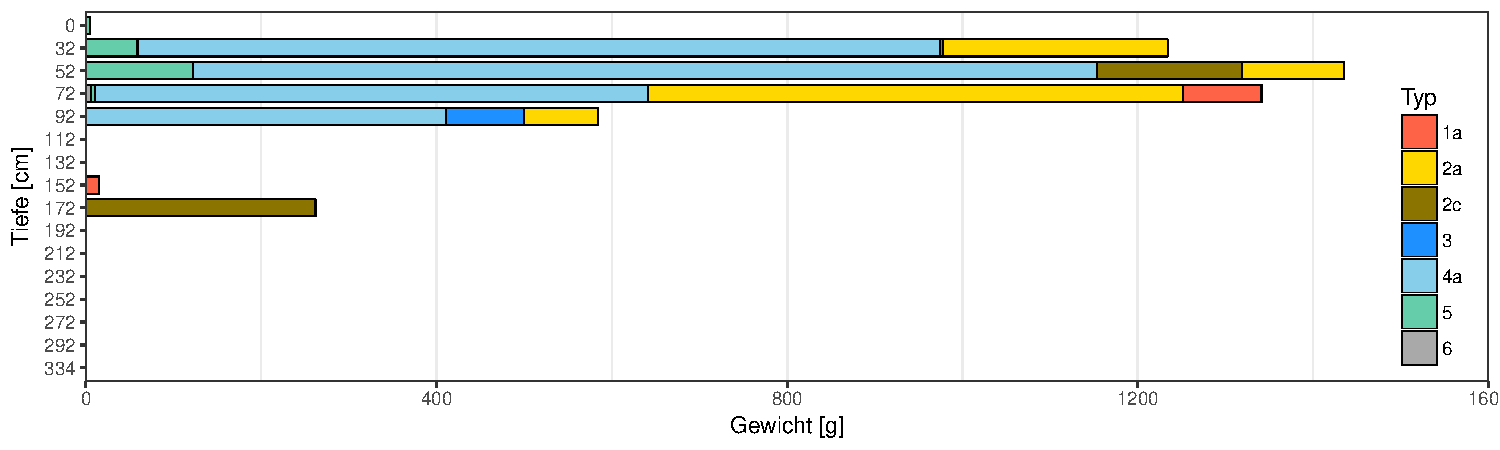
\includegraphics[width = \textwidth]{fig/9-8_PIK87-1_Schlacken_R.pdf}
		\caption{Schlacken.}
		\label{fig:PIK87-1_Schlacken}
	\end{subfigure}
	\caption{PIK~87/1: Verteilung der Fundmaterialien (A), keramischen Stilgruppen (B), \textit{Fabrics} (C) und Schlacken (D) in den entsprechenden Tiefen der Grabung.}
	\label{fig:PIK87-1_KeramikVerteilung}
\end{figure*}

\begin{figure*}[tb!]
	\centering
	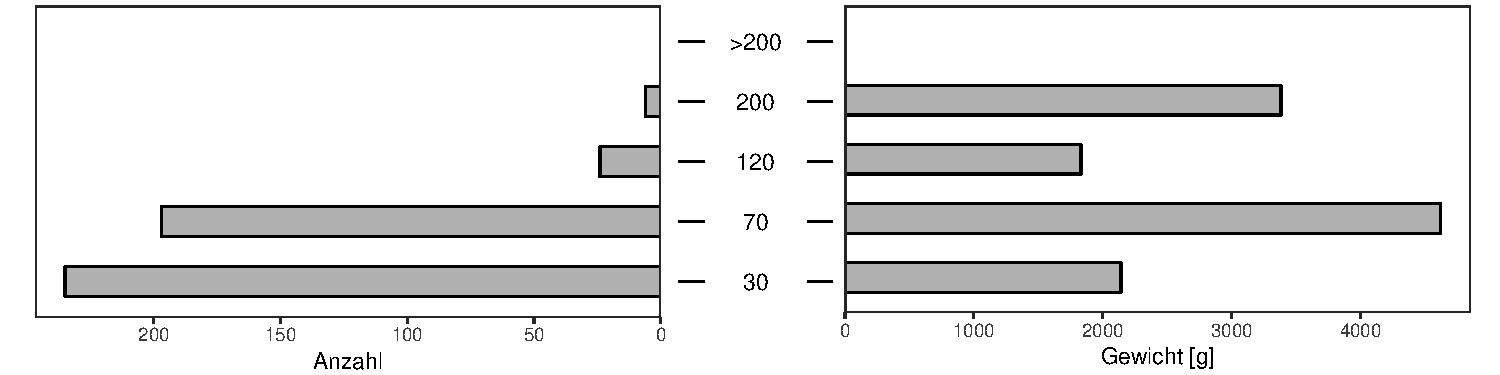
\includegraphics[width=\textwidth]{fig/9-08_PIK87-1_Fragmentierung_2.pdf}
	\caption{PIK~87/1: Fragmentierungsgrad der Scherben (n~=~462; Größenklassen siehe Anm.~\ref{ftn:Keramik_Fragmentierung}).}
	\label{fig:PIK87-1_Fragmentierung}
\end{figure*}

Die Inventare beider Gruben zeigen eine vergleichbare Fragmentierung. Das Gros (80--90\,\%) bilden kleine bis mittelgroße Fragmente, die kleiner als 70\,$\times$\,70\,mm sind (Abb.\ref{fig:PIK87-1_Fragmentierung}). Nur in den oben bereits erwähnten Abträgen 3--4 und 8--9 fanden sich große Fragmente von Gefäßen, die größer als 120\,$\times$\,120\,mm sind. Da das Fundaufkommen nahe der Grubensohle -- dem Bereich B2 -- stark abnimmt, sind belastbare Aussagen über die Fragmentierung in dieser Zone kaum möglich. Generell ist die Funddichte in der Pikunda-Munda-Keramik-enthaltenden Grube B sehr gering. Die Verteilung der keramischen Stilgruppen spiegelt die beiden erfassten Gruben ebenfalls wider (Abb.~\ref{fig:PIK87-1_VerteilungStilgr}). Im oberen, die Abträge 1--5 umfassenden, Bereich A dominieren Gefäße mit stark geschweifter Wandung, kurzen Zylinderhälsen und ausbiegenden Rändern des Mandombe-Stils (Kap.~\ref{sec:MDB-Gr}). Erst weiter unterhalb finden sich Fragmente von Schalen mit Bauchknick des Pikunda-Munda-Stils (Kap.~\ref{sec:PKM-Gr}). 

\begin{table*}[tb]
	\centering
	{\footnotesize \begin{sftabular}{@{}lrrrrrr@{}}
			\toprule 
			\textbf{Stilgruppe} & \textbf{Gefäß} & \textbf{Rand} & \textbf{Wand} & \textbf{Boden} & \textbf{Summe} & \\ 
			\midrule 
			Mandombe & 2 & 22 & 80 & & 104 & 54,45\,\% \\ 
			fraglich Mandombe & & 46 & 29 & 3 & 78 & 40,84\,\% \\ 
			Konda & & 1 & 1 & & 2 & 1,05\,\% \\ 
			Pandama & & & 2 & & 2 & 1,05\,\% \\ 
			Ebambe & & & 1 & 1 & 2 & 1,05\,\% \\ 
			Matoto & & 2 & & & 2 & 1,05\,\% \\ 
			Mbenja & & & 1 & & 1 & 0,52\,\% \\ 
			\midrule
			Summe & 2 & 71 & 168 & 4 & 245 & \\ 
			\bottomrule 
	\end{sftabular} }
	\caption{PIK~87/1 (A): Anteil Scherben der verschiedenen Gefäßbereiche nach Stilgruppen.}
	\label{tab:PIK87-1A_Keramik_Scherben}
\end{table*}

\paragraph{Keramikinventar in Grube A\vspace{.5em}}\mbox{}\\
\begin{tabular}{@{}lr@{}}
Bearbeitet & \\ 
\hline 
Keramik der Mandombe-Gruppe: & 7056\,g \\ 
Sonstige Stilgruppen in Grube A: & 96\,g \\ 
 & \\ 
1987 Ausgesondert & \\ 
\hline 
\begin{tabular}[c]{@{}l@{}}\textit{rau}-wandige Keramik\\ (potenziell Mandombe-Gruppe)\end{tabular} & 6500\,g \\ 
\end{tabular} 		

\vspace{1em}
\noindent Die oberen Abträge erbrachten eine sehr charakteristische und formal wie technisch homogene Keramik, die als Mandombe-Stil beschrieben ist (Kap.~\ref{sec:MDB-Gr}).\footnote{Das Material aus dem Befund diente als das definierende Spektrum für die Beschreibung des Mandombe-Stils (Kap.~\ref{sec:MDB-Gr}). Um eine Verwechslung mit dem Pikunda-Munda-Stil, der von \textcite{Eggert.1992} als Keramikgruppe eingeführt wurde, zu vermeiden, wurde ein anderer, aussagefähiger Komplex für die Bennung gesucht. Entsprechende Keramik wurde in keiner anderen Grabung erfasst. Die Oberflächenabsammlung von Mandombe am \mbox{Sangha} (Fpl.~259) enthielt jedoch entsprechendes Material und wurde daher für die Benennung der Stilgruppe ausgewählt.} Sie hebt sich vom ansonsten in der Grabung freigelegten Fundspektrum deutlich ab. Keramik des Mandombe-Stils beschränkt sich auf die in den Profilen beobachtete Tiefe der Grube A und obwohl im Feld keine Trennung der Funde nach den Befunden möglich war, kann als starke Hypothese gelten, dass die Mandombe-Keramik aus Grube A stammt.

Das Inventar besteht aus 13~GE die sicher der stark bauchigen Gefäßform D1\footnote{Das Verhältnis von Bauch- zu Halsdurchmesser, welches als Maß der \textit{Bauchigkeit} gelten kann, liegt zwischen 1,5--2,6; die Werte spiegeln somit leicht bis stark bauchige Gefäße wider. Ein signifikanter Kolmogorow-Smirnow-Test unterstreicht eine zweigipfelige Verteilung, mit dezidiert schwach sowie stark bauchigen Gefäßen. Es scheint kein kontinuierliches Spektrum zwischen Gefäßen mit weniger oder solchen mit stark geschweifter Wandung zu geben. Jedoch beruht diese Beobachtung lediglich auf einer geringen Stichprobengröße.} zugeordnet werden können und 16 weiteren GE, die nicht gut genug erhalten waren, um eine eindeutige Ansprache zu ermöglichen.\footnote{Aufgrund der starken Fragmentierung (Abb.~\ref{fig:PIK87-1_Fragmentierung}) war häufig nur eine eingeschränkte Ansprache der Gefäßform möglich.} Es fanden sich keine Scherben, die einer anderen Gefäßform zugerechnet werden könnten. Ränder sind durchweg kurz und ausbiegend, mit einer gerillten Mündung und gehen in typisch kurze, zylindrische Hälse über. Die Schulterbereiche sind stark abgesetzt, häufig mit einem scharfen Knick an der Innenseite. Die Verzierungen der Keramik des Mandombe-Stils unterscheiden sich deutlich von jener der Pikunda-Munda-Keramik aus der älteren Grube B. Im ersten und zweiten Abtrag fand sich jeweils eine mit \textit{knotted strip}-Roulette (Tab.~\ref{tab:Verzierungselemente}: 21.1) verzierte Scherbe. Beide Stücke entsprechen in ihren weiteren formalen Charakteristika dem ansonsten nicht rouletteverzierten Mandombe-Material. Das früheste Auftreten von Rouletteverzierung im Arbeitsgebiet muss auf Basis dieses Fundes in das 12.--14.~Jh. n.~Chr. datiert werden.

Die in Grube A gemachten Funde deuten eine höhere Funddichte an, als in der älteren Grube B. In der kleineren Grube A fand sich zusammengenommen mehr Keramik, als in der etwa dreimal so tiefen Grube B. Zusätzlich enthielt die Grube noch fast 4,6\,kg Schlacke (Abb.~\ref{fig:PIK87-1_VerteilungFunde}). Das Inventar zeigt keine Anzeichen einer planmäßigen Deponierung von Objekten. Es wurden weder vollständige Gefäße gefunden, noch sind größere Zusammensetzungen möglich gewesen. Keine der in die Grube gelangten GE repräsentiert ein ganzes Gefäß.

\paragraph{Sonstige Stilgruppen in Grube A}\hspace{-.5em}|\hspace{.5em}%
Unter dem Material aus den oberen Abträgen fanden sich neben der Keramik des Mandombe-Stils einige Scherben anderer keramischer Gruppen. Diese machen weniger als 3\,\% des insgesamt der Grube A zugewiesenen Materials aus. Eine mit der für die Ebambe-Gruppe (Kap.~\ref{sec:EBA-Gr}) typischen \textit{banfwa-nfwa}-Verzierung versehene Bodenscherbe und eine entsprechend verzierte Wandungsscherbe fanden sich im zweiten Abtrag. Beide Stücke weisen keine nicht-plastischen Partikel im Scherben auf (\textit{Fabric}~1). Zudem fanden sich eine Reihe Wandungsscherben mit \textit{banfwa-nfwa}-Verzierung, die technisch der Keramik der Mandombe-Gruppe ähneln und das \textit{Fabric}~3 aufweisen.\footnote{Ob es sich bei den genannten Stücken mit \textit{Fabric}~1 um einen \textit{Import} handelt und die Scherben mit \textit{banfwa-nfwa}-Verzierung und \textit{Fabric}~3 Teil einer lokalen Produktion sind, muss gegenwärtig offenbleiben.} Darüber hinaus fanden sich vereinzelte Scherben, die Ähnlichkeiten zu den Stilen Matoto (Kap.~\ref{sec:MAT-Gr}), Konda (Kap.~\ref{sec:KON-Gr}), Pandama (Kap.~\ref{sec:PDM-Gr}) und Mbenja (Kap.~\ref{sec:MBJ-Gr}) aufweisen (Abb.~\ref{fig:PIK87-1_VerteilungStilgr}). 

\begin{table*}[tb]
	\centering
	{\footnotesize	\begin{sftabular}{@{}m{.05\textwidth}m{.3\textwidth}m{.3\textwidth}m{.05\textwidth}m{.18\textwidth}@{}}
			\toprule
			\textbf{Nr.} & \textbf{Außenseite/Oberfläche} & \textbf{Anschliff (Profil)} & \textbf{\textit{Fabric}} & \textbf{Objekt} \\
			\midrule
			1 & 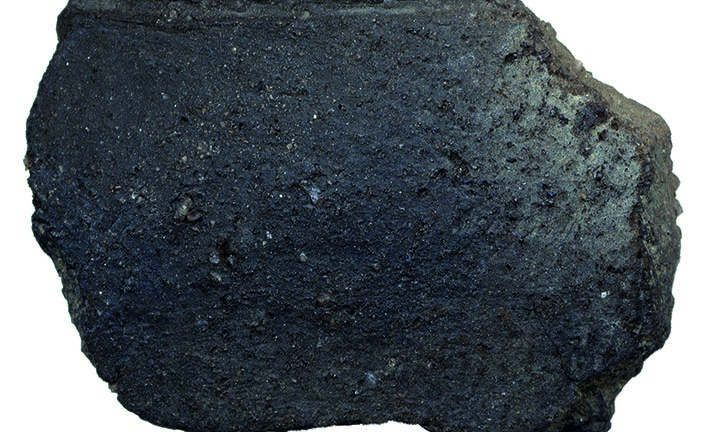
\includegraphics[width=.3\textwidth]{tbl/Tab_Fabrics/PIK87-1-8-1_5cm.jpg} & 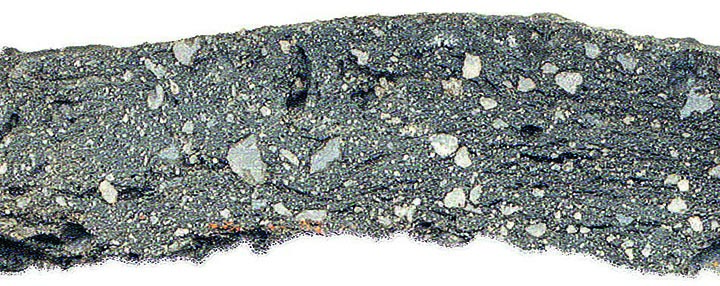
\includegraphics[width=.3\textwidth]{tbl/Tab_Fabrics/PIK87-1-8-1_2cm.jpg} & 10a & PIK~87/1-8:1 \\
			2 & 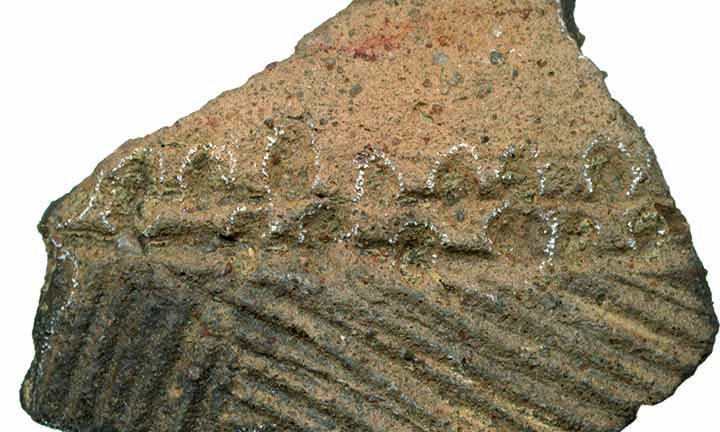
\includegraphics[width=.3\textwidth]{tbl/Tab_Fabrics/PIK87-1-8-2_5cm.jpg} & & 4b & PIK~87/1-8:2 \\
			3 & 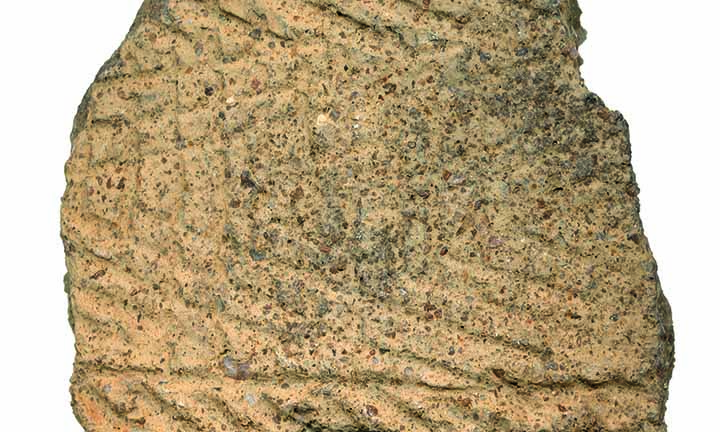
\includegraphics[width=.3\textwidth]{tbl/Tab_Fabrics/PIK87-1-9-7_5cm.jpg} & 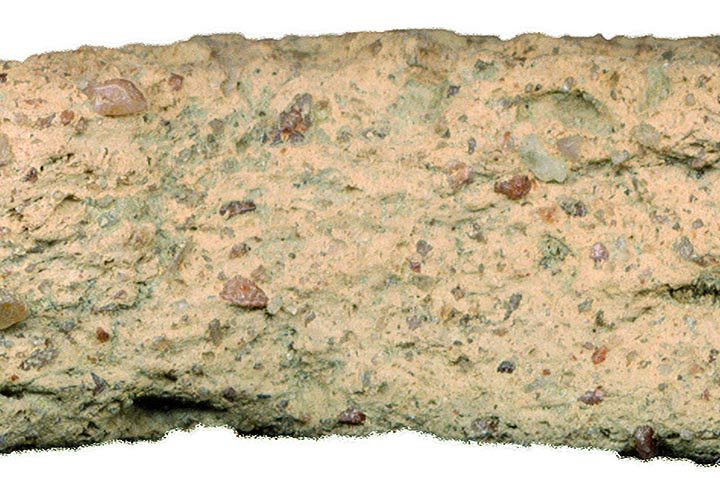
\includegraphics[width=.3\textwidth]{tbl/Tab_Fabrics/PIK87-1-9-7_2cm.jpg} & 4b & PIK~87/1-9:7 \\
			& 
\includegraphics[width=.3\textwidth, page = 1]{tbl/Tab_Fabrics/x_fabrics_scales.pdf} & 
\includegraphics[width=.3\textwidth, page = 2]{tbl/Tab_Fabrics/x_fabrics_scales.pdf} & & \\
			\bottomrule
	\end{sftabular} }
	\caption{PIK~87/1 (B1): Scherben aus dem mittleren Abschnitt des Grubenteils B1, die nicht der Pikunda-Munda-Gruppe zugeordnet werden können.}
	\label{tab:PIK87-1bis9_nichtPIK-MUN}
\end{table*}

\begin{table*}[tb]
	\centering
	{\footnotesize \begin{sftabular}{@{}lrrrrrr@{}}
			\toprule 
			\textbf{Stilgruppe} & \textbf{Gefäß} & \textbf{Rand} & \textbf{Wand} & \textbf{Boden} & \textbf{Summe} & \\ 
			\midrule 
			Pikunda-Munda & 2 & 37 & 102 & 1 & 142 & 86,59\,\% \\ 
			fraglich Pikunda-Munda & & 1 & 16 & & 17 & 10,37\,\% \\ 
			fraglich \mbox{Ngbanja} & & & 3 & 1 & 4 & 2,44\,\% \\ 
			Lusako & & 1 & & & 1 & 0,61\,\% \\ 
			\midrule 
			Total & 2 & 39 & 121 & 2 & 164 & \\ 
			\bottomrule 
	\end{sftabular}}
	\caption{PIK~87/1 (B1/B2): Anteil Scherben der verschiedenen Gefäßbereiche nach Stilgruppen.}
	\label{tab:PIK87-1B1B2_Keramik_Scherben}
\end{table*}

\paragraph{Keramikinventar in Grube B1/B2\vspace{.5em}}\mbox{}\\
\begin{tabular}{@{}lr@{}}
Bearbeitet & \\ 
\hline 
Keramik der Pikunda-Munda-Gruppe: & 4415\,g \\ 
Sonstige Stilgruppen in Grube B: & 135\,g \\ 
 & \\ 
1987 Ausgesondert & \\ 
\hline 

\begin{tabular}[c]{@{}l@{}}\textit{glatt}-wandige Keramik\\ (potenziell Pikunda-Munda-Gruppe)\end{tabular} & 1690\,g \\ 
\begin{tabular}[c]{@{}l@{}}\textit{rau}-wandige Keramik\\ (potenziell \mbox{Ngbanja}-Gruppe)\end{tabular} & 190\,g \\ 
\end{tabular} 		

\vspace{1em}
\noindent Die Keramik aus Grube B ist ebenfalls stark fragmentiert. Es fand sich lediglich eine nahezu komplette (Taf.~44.3) sowie eine teilweise erhaltene Schale (Taf.~45.2) der Pikunda-Munda-Gruppe in den Abträgen 7--9.\footnote{Die fast vollständige Schale lag bei der Grabung nicht im Verband, sondern war bereits zerscherbt und in der Grubenfüllung verteilt. Die Einzelteile fanden sich in zwei Abträgen und im zu Beginn ausgehobenen Profilkasten (Abb.~\ref{fig:PIK87-1_PlanaSkizze}; \ref{fig:PIK87-1_ProfileZeichnung}).}

Eine zentrale Frage an die Auswertung der Keramik aus Grube B bestand darin, abzuklären, ob sich zwischen dem Fundgut aus den beiden Bereichen B1 und B2 Unterschiede erkennen lassen.\footnote{Aus der Befunddokumentation ist nicht ersichtlich, bis zu welchem Grad die Bereiche B1 und B2 eigenständige Befunde repräsentieren. Unterschiede in der Keramik der beiden Bereiche könnten ein Indikator für zwei potenziell eigenständige Inventare sein.} Im unteren Bereich B2 finden sich keine Fragmente klassischer Pikunda-Munda-Schalen mit deutlichen Bauchknick vom Typ F3. Im oberen Bereich B1 konnte nur die nahezu vollständig erhaltene Schale sicher diesem Typ zugewiesen werden (Taf.~44.3). Daneben fanden sich bis zum neunten Abtrag (T~192) Fragmente von zehn GE, die grundsätzlich als Schalen des Typs F3 beziehungsweise E3 angesprochen werden konnten. Die zweite identifizierbare Gefäßform, leicht bauchige Gefäße mit ausbiegendem Rand und ohne ausgeprägten Hals vom Typ E1, sind über nahezu alle Abträge verteilt. Da das Material stark fragmentiert ist, war eine Ansprache der Gefäßform jedoch häufig nicht möglich. Ein Vergleich der beobachteten Mündungsabschlüsse sowie der Randformen erbrachte ebenfalls keine klaren Unterschiede zwischen den beiden Bereichen. Fast alle erfassten Ränder sind ausbiegend (80\,\%). Etwa 40\,\% sind gerade (Typ B1) und weitere 30\,\% konvex ausbiegend (Typ B3). Etwa die Hälfte der Mündungen sind gerade abgestrichen (M3). Die Keramik aus dem unteren Grubenteil B2 bildet, vor allem aufgrund des geringeren Fundaufkommens, lediglich ein verarmtes Spektrum der Anteile von Formen und Verzierungen des oberen Bereichs B1 ab.

Gefäße mit geschweifter Wandung vom Typ E1 sind, im Unterschied zu Schalen des Typs F3, selten flächig verziert. Häufig finden sich Bänder aus Schraffurmustern oder horizontalen Rillen, eingefasst von Reihen aus Eindrücken auf den Gefäßbäuchen. Die für die Pikunda-Munda-Gruppe typischen Schalen mit Bauchknick vom Typ F3 aus dem Inventar der Grabung PIK~87/1 sind dagegen häufiger flächig verziert und zeigen Reihen aus horizontalen Eindrücken eher selten. Das Gros der Verzierungselemente bilden kammstrichähnliche Verzierungen, gefolgt von Reihen aus Eindrücken und flächigen Schachbrett-Mustern. Mehr als 90\,\% der Pikunda-Munda-Keramik weist das \textit{Fabric}~1 auf, welches sich durch keine oder kaum Zusätze mit nichtplastischen Partikeln auszeichnet.\footnote{Der Rest des Materials kann -- bis auf zwei Scherben -- dem \textit{Fabric}~2 zugeordnet werden, das sich vom \textit{Fabric}~1 nur durch die Nutzung rotbrennender Tone unterscheidet. Die entsprechenden Scherben weisen in keinem Fall eine stark rote Färbung auf. Auch verteilen sie sich ebenfalls gleichmäßig auf beide Grubenteile. Das Gros der weißbrennenden Keramik zeigt eine randliche Oxidation mit einem dunklen Kern und ist der Variante 1b zuzuordnen (\textasciitilde40\,\%). Ebenfalls zahlreich finden sich Stücke mit einer tiefer greifenden Oxidation und dementsprechend schwachem Restkern der Variante 1d (\textasciitilde20\,\%). Diese Effekte des Brandes können jedoch auf einzelnen Gefäßen deutlich unterschiedlich ausgeprägt sein. Eine Differenzierung beziehungsweise Unterscheidung der beiden Bereiche B1 und B2 ergab sich auch bei den technischen Charakteristika des Materials nicht.}

\paragraph{Sonstige Stilgruppen in Grube B1}\hspace{-.5em}|\hspace{.5em}%
Im achten und neunten Abtrag fanden sich Scherben, die nicht in das Spektrum der Pikunda-Munda-Gruppe einzuordnen sind (Abb.~\ref{fig:PIK87-1_VerteilungStilgr}). Es handelt sich um Formen, die auffällige Ähnlichkeiten zur \mbox{Ngbanja}-Keramik des mittleren \mbox{Ubangi} aufweisen. Besonders für eine Scherbe  mit flacher plastischer Leiste und kleinen runden Eindrücken (Tab.~\ref{tab:PIK87-1bis9_nichtPIK-MUN}.1; Taf.~47.20) findet sich in \mbox{Ngbanja} am \mbox{Ubangi} (Fpl.~199) eine nahezu exakte Entsprechung (Taf.~6.9; siehe Kap.~\ref{sec:NGB-Gr}).

Am Übergang des oberen Bereichs B1 zum unteren Grubenteil B2, der sicher ab dem 13. Abtrag (T~\textless\,252) erfasst wurde, fand sich ein weiteres Stücke, das nicht der Pikunda-Munda-Gruppe zugeordnet werden konnte. Es handelt sich um eine Scherbe der aus dem östlich angrenzenden Inneren Kongobecken bekannten Lusako-Gruppe \parencites[Taf.~45.16;][18 Abb.~4.1]{Eggert.1992}[104--107]{Wotzka.1995}. Die Scherbe kann prinzipiell zum Grubenteil B2 gehören, ebenso aber auch noch an der Sohle des Grubenteils B1 gelegen haben. Das Stück weist, wie auch die mit ihr gefundene Pikunda-Munda-Keramik, das \textit{Fabric}~1 auf. Bereits \textcite[107]{Wotzka.1995} weist auf die \enquote{formalen und ornamentalen Gemeinsamkeiten [der Pikunda-Munda-Keramik] mit den Stilgruppen Lokondola, Lusako, Lingonda und Bokuma} des von ihm untersuchten Inneren Kongobeckens hin (siehe Tab.~\ref{tab:PIKMUN_Vgl}).

\paragraph{Keramische Sonderformen}\hspace{-.5em}|\hspace{.5em}%
In den ersten beiden Abträgen fanden sich einige kleine Stücke gebrannten Lehms und im vierten Abtrag weitere Stücke mit konkaven Abdrücken, die von Stangen mit Durchmessern von 5\,cm sowie 20\,cm herrühren. An der Sohle der Grube fand sich überdies ein größeres Stück gebrannten Lehms.

Erwähnenswert sind überdies zwei Tonzylinder, einer wurde im 13. Abtrag, nahe der Sohle, gefunden und der zweite direkt an der Sohle. Der im 13. Abtrag gefundene Tonzylinder hatte einen Durchmesser von 13\,mm und war etwa 20\,mm lang. Bei dem an der Grubensohle gefundenen Objekt handelt es sich um ein schwach oder nicht gebranntes Stück, das im Profil fünfeckig war. Die Seitenflächen sind knapp 20\,mm breit. Das Stück war bereits stark zerfallen und nur noch etwa auf einer Länge von etwa 50\,mm erhalten. Für beide Objekte können derzeit weder Funktion noch Vergleiche angegeben werden.

\begin{figure*}[tb!]
	\centering
	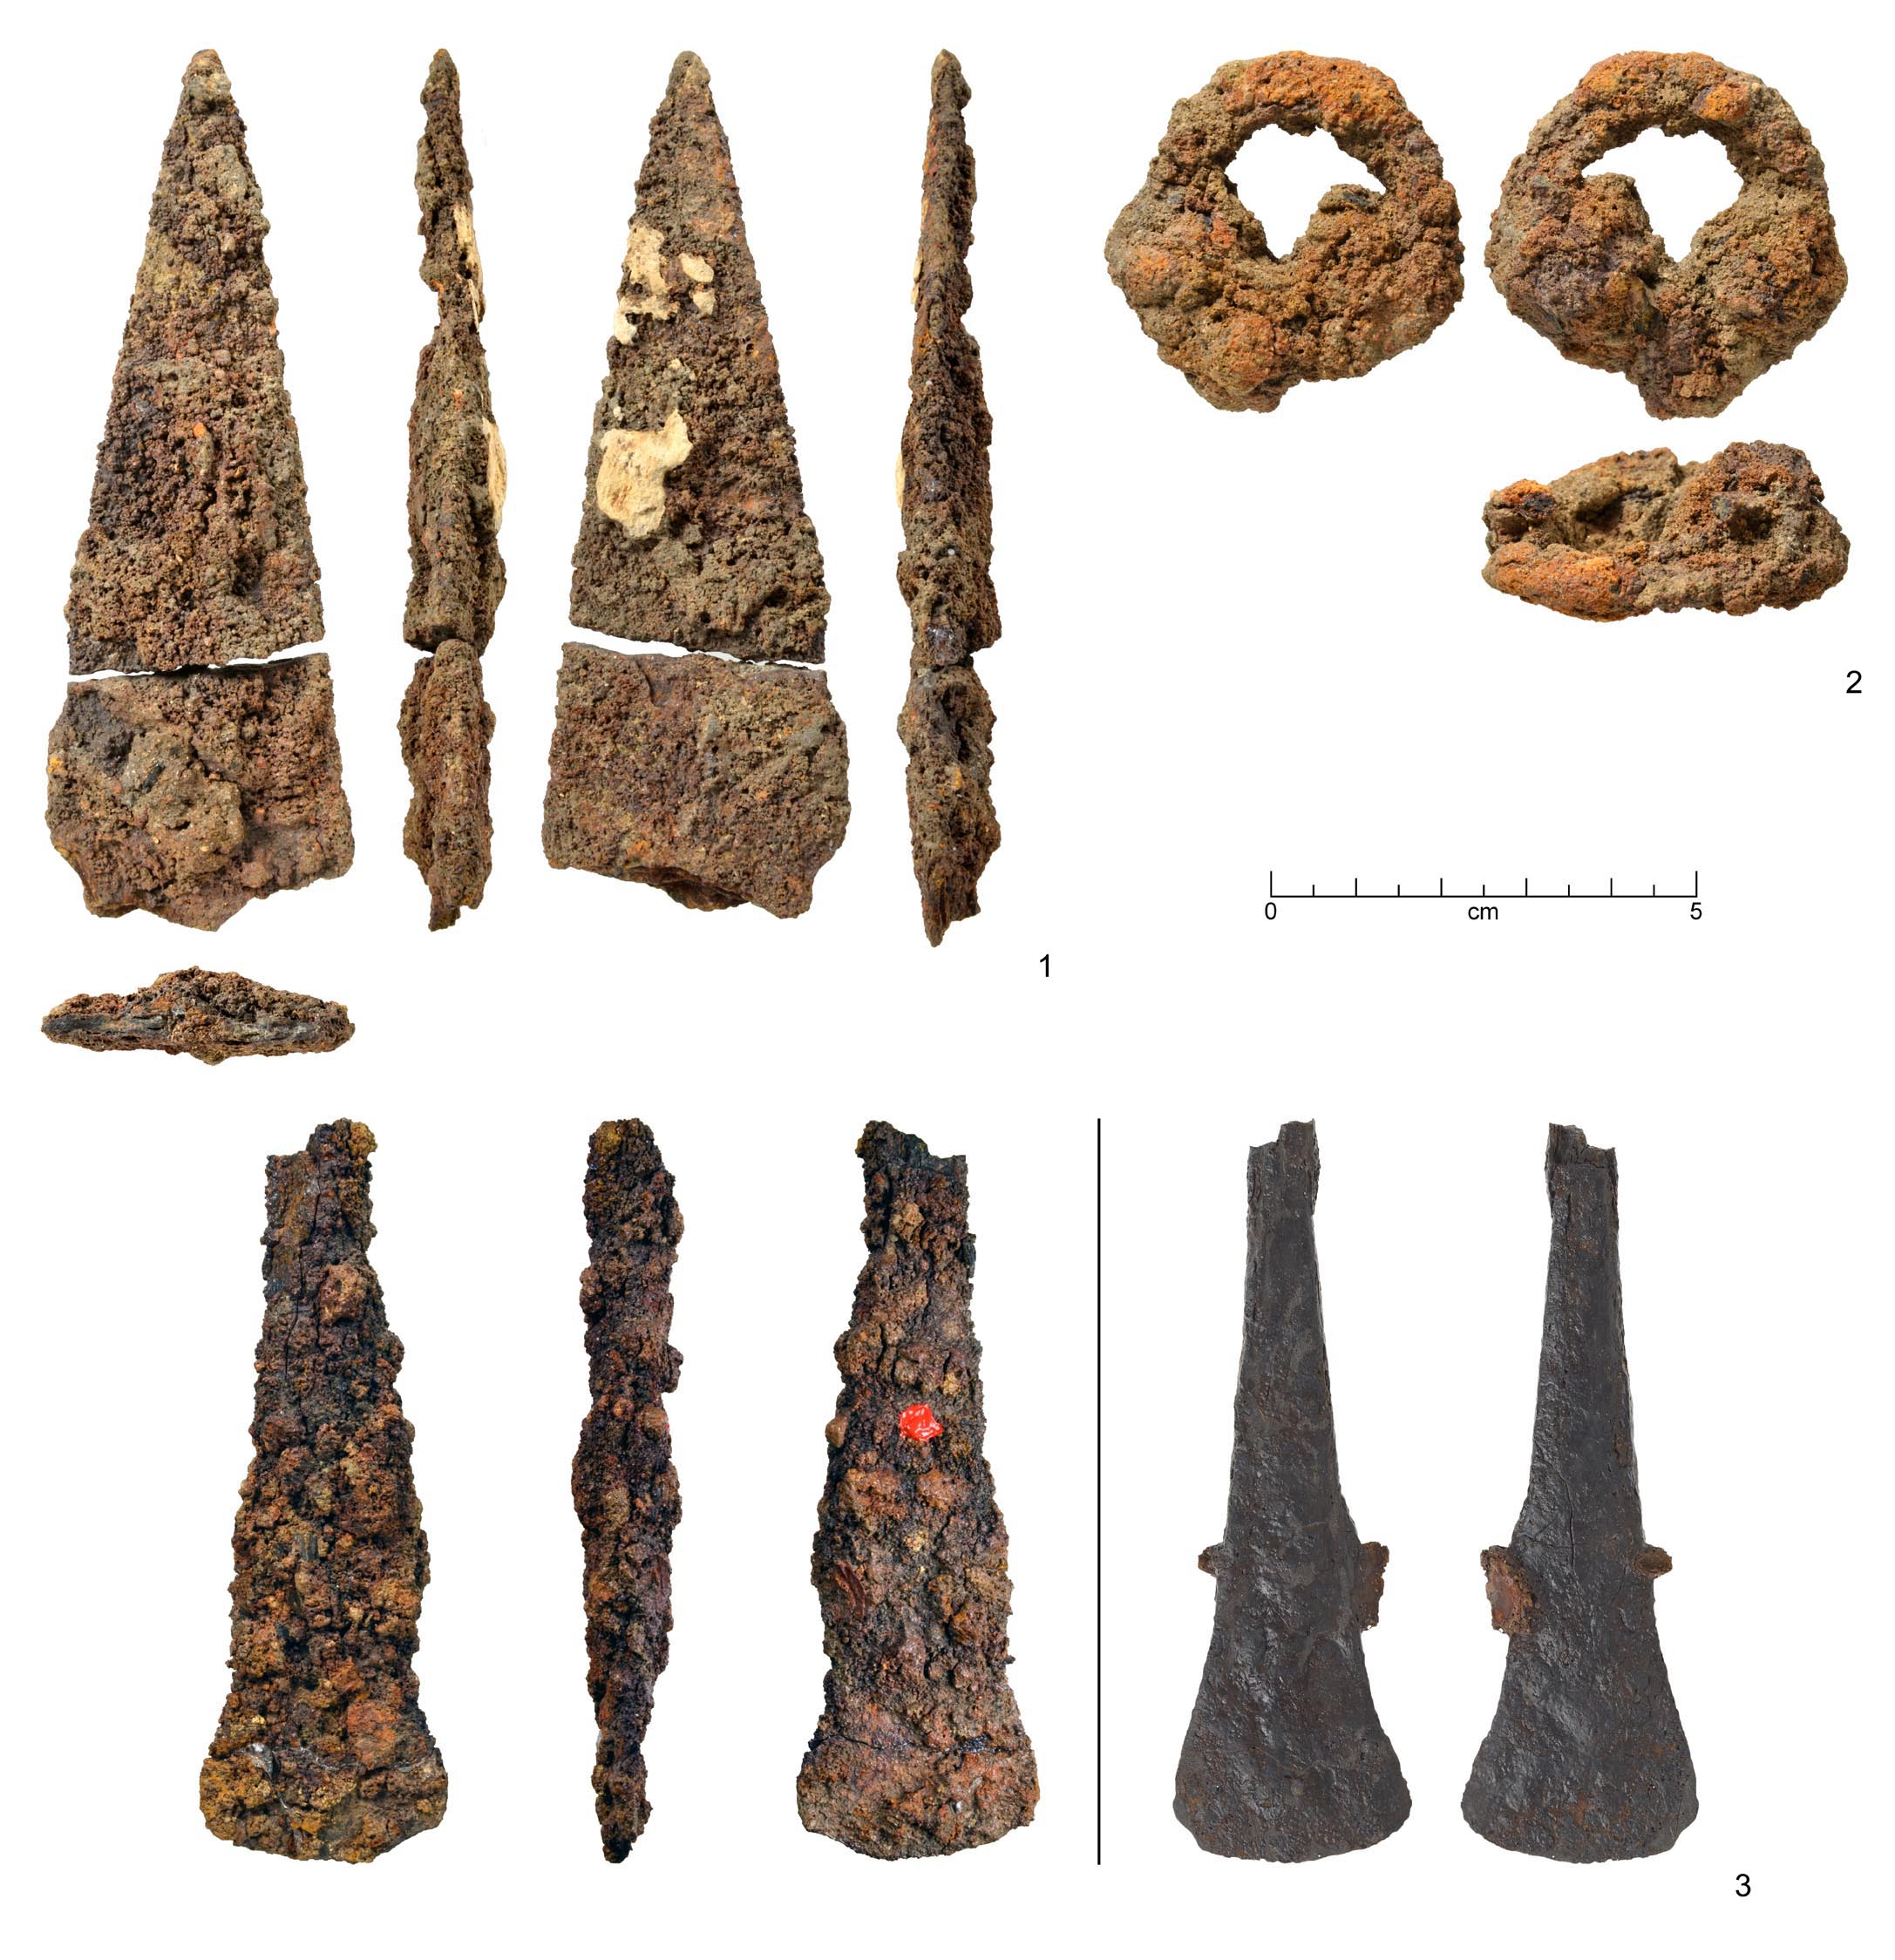
\includegraphics[width=\textwidth]{fig/PIK87-1_Eisen_2014-01-17.jpg}
	\caption{PIK~87/1: Eisenfunde. 1: Obj. PIK~87/1-2 aus Abtrag 2; 2: Obj. PIK~87/1-7 aus Abtrag 7; 3: Obj. PIK~87/1-9 aus Abtrag 9. Fotos 1--3 zeigen den Zustand vor der Restaurierung (Fotos: D. Seidensticker) und 3 auch den restaurierten Zustand (Foto: R. Müller/RGZM, 2012).}
	\label{fig:PIK87-1_Eisen}
\end{figure*}

\paragraph{Sonstige Funde}\hspace{-.5em}|\hspace{.5em}%
Im zweiten Abtrag fand sich eine mögliche Geschoss- oder Lanzenspitze aus Eisen (Abb.~\ref{fig:PIK87-1_Eisen}.1). Direkt vor dem Ostprofil und eindeutig zum Grubenteil B1 gehörend fanden sich im siebten Abtrag zwei oder eventuell auch drei zusammenkorrodierte Eisenringe (Abb.~\ref{fig:PIK87-1_ProfileZeichnung}). Sie bestehen aus etwa 5\,mm breitem und 2\,mm dickem, im Querschnitt quadratischem Draht und weisen einen Durchmesser von etwa 30\,mm auf (Abb.~\ref{fig:PIK87-1_Eisen}.2).

Etwas unterhalb der Ringe, im neunten Abtrag, wurde ein kleines eisernes Beil gefunden (Abb.~\ref{fig:PIK87-1_Eisen}.3).\footnote{Das Stück wurde zusammen mit Eisenobjekten aus dem früheisenzeitlichen Friedhof von Campo \parencite[Südkamerun; ][]{Eggert.2016} sowie einem aus Munda stammenden Stück (Abb.~\ref{fig:MUN87.2-1-1-2_Eisengeld_Foto}) am Römisch-Germanischen Zentralmuseum in Mainz (RGZM) restauriert.} Der Schaft des Beils hat einen rechteckigen Querschnitt und weist eine unregelmäßige Bruchkante auf. Die Schneide ist angeschärft und leicht gerundet. Die Ecken sind deutlich abgerundet, was auf eine aktive Nutzung zurückgeführt werden kann. Die Schneide ist zirka 22\,mm breit und das Beil noch bis zu einer Länge von etwa 85\,mm erhalten. Es zeigt an zwei Stellen Abdrücke von ehemals organischem Material, das jedoch nicht näher bestimmt werden kann.\footnote{Mündl. Mitt. S. Ritter (RGZM, Mainz 2014).}

\begin{figure*}[!tb]
	\begin{minipage}{\textwidth}
		\centering
		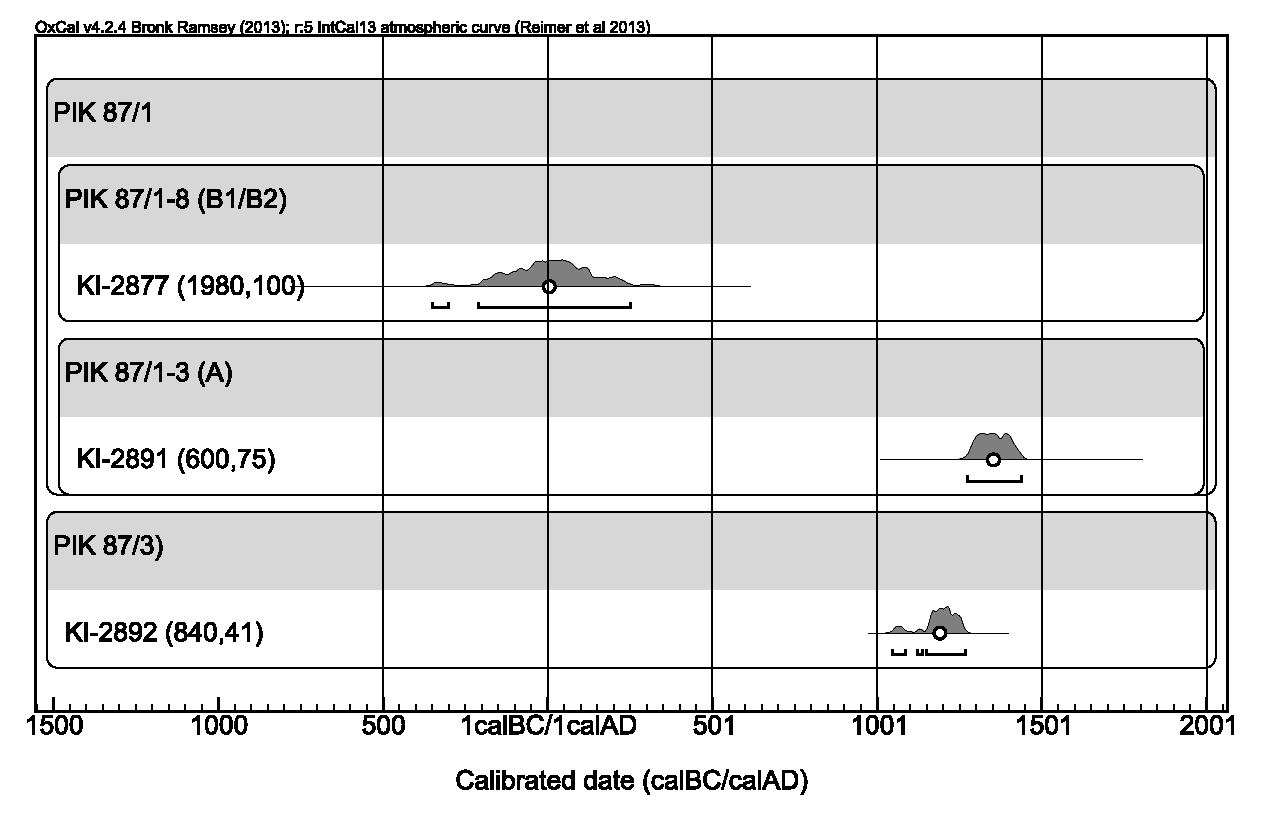
\includegraphics[width=.75\textwidth]{fig/PIK87_14C.pdf}
		\captionof{figure}{Pikunda: Kalibrierte \textsuperscript{14}C-Datierungen aus dem Schnitt PIK~87/1 sowie aus dem Metallurgie-Befund PIK~87/3 (Kat.-Nr.~10).}
		\label{fig:PIK87_Datierungen}
	\end{minipage}
	
	\vspace{2em}
	
	\begin{minipage}{\textwidth}
		{\footnotesize
			\centering
			\begin{sftabular}{@{}p{.1\textwidth}p{.1\textwidth}p{.3\textwidth}p{.2\textwidth}p{.15\textwidth}@{}}
				\toprule
				\textbf{Lab-Nr} & \textbf{Datum (bp)} & \textbf{Datum (2-Sigma)} & \textbf{Abtrag} & \textbf{Tiefe (unter NP)} \\ 
				\midrule
				KI-2877 & 1980\( \pm \)100 & \parbox[t]{.25\textwidth}{351--302 v.~Chr. (2,2\,\%)\\210 v.~Chr.--252 n.~Chr. (93,2\,\%)} & Abtrag 8 (HK 11) & 1,52--1,72\,m \\ 
				KI-2891 & 600\( \pm \)75 & 1276--1437 n.~Chr. & Abtrag 3 (HK 7) & 0,57\,m \\ 
				\bottomrule 
		\end{sftabular}}
		\captionof{table}{PIK~87/1: \textsuperscript{14}C-Datierungen.}
		\label{tab:PIK87-1_Datierungen}
	\end{minipage}
\end{figure*}

Das Gros der insgesamt fast 4,6\,kg Eisenschlacke, die in der Grabung gefunden wurden, stammt aus den obersten vier Abträgen (Abb.\ref{fig:PIK87-1_VerteilungFunde}). Etwa 2/3 der gefundenen Schlacken sind kantig, nicht magnetisch und zeigen keine oder nur wenige Fließstrukturen (Tab.~\ref{tab:Schlacken}: Typ 4a). Das restliche Drittel besteht fast vollständig aus Fließschlacken hoher Viskosität des Typs 2a sowie Schlacken mit blau-violetter Farbe des Typs 2c. Im dritten Abtrag kommen Schlacken hoher Viskosität vom Typ 2a und kantige Schlacken vom Typ 4a in etwa zu gleichen Teilen vor. In den obersten Abträgen finden sich einige Stücke mit rost-roter Farbe und einer groben, verbackenen Matrix, die teilweise an Laterit erinnern und dem Schlacken-Typ 5 zugeordnet sind. Grube B können lediglich 277\,g Eisenschlacke eindeutig zugeordnet werden. Es handelt sich um ein kleines Stück wenig magnetischer Schlacke mit deutlichen Fließstrukturen vom Typ~1 (Tab.~\ref{tab:Schlacken}) und ein größeres Stück mit bläulich-violetter Farbe vom Typ~2c.\footnote{Es muss offenbleiben, ob auch Schlacken dieses Typs aus den Abträgen 1--4, in denen Grube B von der jüngeren Grube A geschnitten wurde, ursprünglich der Grube der Pikunda-Munda-Gruppe zuzurechnen sind. Der Fund von Eisenschlacke im Kontext der ins 4.~Jh. v.~Chr.--4.~Jh. n.~Chr. datierenden und mit Keramik des Pikunda-Munda-Stils assoziierten Grube B zählt zu den ältesten Belegen für Eisenmetallurgie im äquatorialen Regenwald Zentralafrikas.}

\paragraph{Tierknochen}\hspace{-.5em}|\hspace{.5em}%
Im ersten Abtrag fand sich das distale Fragment des linken \textit{Humerus} eines Buntbocks (\textit{Damaliscus pygargus}) oder einer Damagazelle (\textit{Nanger dama}/\textit{Gazella dama}).\footnote{Da die beiden Arten des Buntbockes \textit{D. pygargus pygargus} sowie \textit{D. pygargus phillipsi} rezent im südlichen Afrika verbreitet sind \parencites[siehe][42 Abb.~28]{Boshoff.2016}[2\,f. Abb.~1, Tab.~1, Abb.~2]{Radloff.2016}, die Damagazelle jedoch in der nördlichen Sahelzone und südlichen Sahara heimisch ist \parencite[siehe][2 Abb.~1]{Senn.2014}, kann eine Zuweisung zu letzterem als wahrscheinlicher gelten.} Im achten Abtrag wurde das Fragment der Wurzel eines Elefantenzahnes gefunden.\footnote{Nach Tagebucheintrag von M.~K.~H.~Eggert vom 11.\,06.\,1987 handelt es sich um einen kleinen \textit{Zusatz}-Zahn aus dem Unterkiefer eines Elefanten.} Im Bereich der Sohle, im 13. Abtrag, fanden sich neben einigen kleinen \textit{Vertebrae} eines großen Barsches (\textit{Lates}) noch Fragmente einer linken \textit{Fibula}, die sich einer großen Antilopenart, möglicherweise einer Elenantilope (\textit{Taurotragus oryx}), zurechnen lässt.\footnote{Für die Bestimmung der Tierknochen danke ich Monika Doll, Angelika Wilk (beide Tübingen) und Veerle Linseele (Löwen).}

\paragraph{Datierung}\hspace{-.5em}|\hspace{.5em}%
Aus den drei Grubenbereichen A, B1 und B2 lagen jeweils dezidierte Datierungsproben vor. Allerdings wiesen nur die Proben aus der mit Mandombe-Keramik assoziierten Grube A sowie jene aus dem Pikunda-Munda-Keramik aufweisenden Grubenbereich B1 ausreichend Kohlenstoff für eine -- seinerzeit noch konventionelle -- Radiokolhenstoffdatierung auf (Tab.~\ref{tab:PIK87-1_Datierungen}, Abb.\ref{fig:PIK87_Datierungen}). Grube A kann mittels einer Probe aus dem dritten Abtrag (KI-2891) in das 12.--14.~Jh. n.~Chr. datiert werden.\footnote{Dieses Datum bildet zum gegenwärtigen Zeitpunkt das einzige absolute Datierungsindiz für die Keramik der Mandombe-Gruppe (Kap.~\ref{sec:MDB-Gr}). Es schließt zeitlich an die Datierung aus dem ebenfalls in Pikunda am \mbox{Sangha} gefundenen Metallurgiebefund PIK~87/3 (Kat.-Nr.~10) an (Abb.~\ref{fig:PIK87_Datierungen}: KIA-2892).} Das Alter von Grube B lässt sich mittels einer weiteren datierten Probe aus dem achten Abtrag (KI-2877) auf einen Zeitraum vom 4.~Jh. v.~Chr.--3./4.~Jh. n.~Chr. eingrenzen. Das Datum stimmt mit den weiteren bekannten Datierungen für den Pikunda-Munda-Stil überein (Kap.~\ref{sec:PKM-Gr}). Zusätzlich zu diesen beiden Proben wurde auch aus dem 14. Abtrag eine Probe zur Radiokohlenstoffdatierung entnommen und eingesandt, eine Datierung war jedoch nicht möglich.\footnote{Die Probe sollte nach einem Schreiben vom Kieler Labor vom 22.\,12.\,1987 ausreichend Kohlenstoff enthalten haben. In einem Schreiben vom 01.\,09.\,1989 erklärt das Labor jedoch, dass doch nicht genügend Kohlenstoff zur Messung vorhanden war. Es erfolgte daher keine Messung und die Proben wurden anschließend vom Labor verworfen.}

\paragraph{Interpretation}\hspace{-.5em}|\hspace{.5em}%
Im Grabungsschnitt PIK~87/1 wurden zwei unterschiedliche Grubenbefunde erfasst. Im oberen Bereich schneidet die Grube A der Mandombe-Gruppe in die bis an die Sohle des Schnitts reichende Grube B der Pikunda-Munda-Gruppe ein. Grube A datiert ins 12.--14.~Jh. n.~Chr. und wurde bis zu einer Tiefe von etwa 1~m unter der rezenten Oberfläche erfasst. Angaben zur Größe beziehungsweise dem Durchmesser des Befundes können nicht gemacht werden, da er durch die Grabung nur randlich angeschnitten wurde. Dies gilt ebenso für die Grube B, die in einen oberen Bereich (B1) und einen unteren (B2) unterschieden werden kann. Die Fundauswertung ergab keine Unterschiede des keramischen Inventars dieser beiden Bereiche.

Die mit Keramik des Mandombe-Stils verfüllte Grube A zeichnet sich durch eine stark mit Funden durchmischte Verfüllung aus. Innerhalb des Inventars ergaben sich jedoch auffällig wenige Zusammensetzungen. Auch enthielt der Befund eine größere Menge Eisenschlacke. Die Funddichte ist insgesamt sehr hoch und liegt bei etwa 45\,kg/m\textsuperscript{3} Keramik und \textgreater\,15\,kg/m\textsuperscript{3} Schlacke. Die Grube B, die mit Pikunda-Munda-Keramik verfüllt ist, weist hingegen nur eine Funddichte von knapp 3\,kg/m\textsuperscript{3} auf; bei einem ausgegrabenen Volumen von etwa 2,4\,m\textsuperscript{3}. Insgesamt wurden durch die Grabung nur etwa 10\,\% der ursprünglichen, in der rezenten Oberfläche sichtbaren runden Verfärbung (Abb.~\ref{fig:PIK87-1_FundstelleObfl_Foto}) untersucht. Die Grenzen der Befunde sind lediglich im Norden -- durch die Erosionsrinne -- erfasst worden. Keine der beiden Gruben weist Indizien auf, die die intentionelle Deponierung der jeweiligen Keramikinventare -- im Sinne von \textcite{Wotzka.1993} -- nahelegen.\footnote{Siehe auch Kap.~\ref{sec:GrabungenBefunde}.}

Nicht sicher abgeklärt werden konnte die Frage, ob die beiden Grubenteile B1 und B2, die beide Keramik der Pikunda-Munda-Gruppe enthielten, zwei getrennte Eingrabungen repräsentieren. Die teilweise Überlagerung des Grubenteils B2 mit anstehendem Lehm (Abb.~\ref{fig:PIK87-1_ProfileZeichnung}: Schicht~10) deutet eine deutliche zeitliche Trennung der beiden Befundteile an. Als mögliche Hypothese für die Genese des Befundes kann gelten, dass die ursprünglich bis auf etwa 3\,m unter der heutigen Oberfläche ausgehobene Grube B2 zum Teil einstürzte oder verfüllt wurde. Der Grubenbereich B1 zeichnet schließlich eine spätere Nutzung nach. Alternativ könnte die ursprünglich ausgehobene Grube B2 auch bereits vollständig verfüllt gewesen sein und zu einer späteren Zeit -- jedoch noch zur Zeit des Pikunda-Munda-Stils -- wurde die durch den Bereich B1 repräsentierte Grube eingetieft.\footnote{Die Tatsache, dass das Substrat der Verfüllung des unteren Grubenteils B2 stark heterogen und kaum mit Funden durchsetzt ist, kann leider nicht als unterstützendes Argument für eine der beiden Hypothesen herangezogen werden, da zum Beispiel die unterste Verfüll-Schicht~1c des Befundes BSN~85/1 in Boso-Njafo am Lulonga ebenfalls annähernd fundfrei war \parencites[382--386]{Wotzka.1995}. Auch die von \textcite[5 Abb.~3, 6 Abb.~5]{LivingstoneSmith.2017} präsentierten Befunde weisen nahezu fundfreie äußere sowie untere Grubenbereiche auf.} Da die Analyse des Fundguts keine Unterschiede zwischen den keramischen Inventaren der Grubenteile B1 und B2 erbrachte, ist ein größerer zeitlicher Abstand zwischen den beiden Bereichen weniger wahrscheinlich.